
\section{三垂线定理}
前面，我们已经研究了直线和平面的各种位置关系. 在直线和平面相交的情况中，我们引入了平面的垂线，平面的
斜线，斜线在平面上的射影等概念。在这个基础上，我们进一步研究直线$\ell$和平面$\alpha$内的直线的位置关系.

当$\ell\bot\alpha$时，对任意的$m\subset\alpha$，有$\ell\bot m$。

当$\ell$和$\alpha$斜交时，$\alpha$内有哪些直线与$\ell$垂直呢？

\begin{thm}
  {三垂线定理} 在平面内的一条直线，如果和这个平面的一条斜线的射影垂直，那么它也和这条斜线垂直.  
\end{thm}

已知：$PA$、$PO$分别是平面$\alpha$的垂线、斜线，$AO$是$PO$在平面$\alpha$上的射影. $a\subset\alpha$, $a\bot AO$（图1.47）

求证：$a\bot PO$

\noindent
\begin{minipage}{.6\textwidth}\CTEXindent
\begin{analyze}
要证明$a\bot PO$，可以证明$a$垂直于$PO$所在的一个平面. 由已知，可取$PO$所在的平面$PAO$. 因为可以证明$a$与平面$PAO$的两条相交直线$PA$、$AO$都垂直. 从而可证$a\bot $平面$PAO$.
\end{analyze}

\begin{proof}
$\because\quad PA\bot \alpha,\quad a\subset\alpha$

$\therefore\quad PA\bot\alpha$，由于$AO\bot\alpha$

$\therefore\quad a\bot$平面$PAO$，由于$PO\subset $平面$PAO$

$\therefore\quad a\bot PO$
\end{proof}
\end{minipage}
\hfill
\begin{minipage}{.38\textwidth}
\centering
\begin{tikzpicture}[]
\tkzDefPoints{-.5/0/a, 3/0/b, 4/1.5/c, 0.5/1.5/d}
\tkzDrawPolygon(a,b,c,d)
\tkzLabelAngle[pos=.4](b,a,d){$\alpha$}
\tkzDefPoints{1/2.5/P, 2/.8/O, 1/.8/A}

\draw[thick](.5,.8)--(3,.8);
\draw[thick](1,.8)--(1,3);
\tkzDefPointWith[linear, K=1.7](P,O) \tkzGetPoint{P'}
\tkzInterLL(P,P')(a,b) \tkzGetPoint{tmp}
\draw[thick](tmp)--(P');
\draw[thick](1,0)--(1,-1);
\tkzDrawLines[add= .2 and 0](P,O) 

\tkzLabelPoints[below](A,O)
\tkzLabelPoints[right](P)

\tkzDefPoints{2.2/0/A1}
\tkzDefPointBy[translation = from a to d](A1) \tkzGetPoint{D1}
\tkzDefPointWith[linear, K=.2](A1,D1) \tkzGetPoint{tmp1}
\tkzDefPointWith[linear, K=.8](A1,D1) \tkzGetPoint{tmp2}
\draw[thick](tmp1)--(tmp2)node[right]{$a$};
\end{tikzpicture}
\captionof{figure}{}
\end{minipage}

由证明过程可知，$a\subset\alpha$，$a$不一定过$O$点. 所以三垂线定理实质上是两条直线（一个与平面$\alpha$斜交，一个在平面$\alpha$内，特殊情况是相交直线）垂直的判定定理.

类似地可以证明：

\begin{thm}
  {三垂线定理的逆定理} 在平面内的一条直线，如果和这个平面的一条斜线垂直，那么它也和这条斜线在这平面上的
射影垂直.  
\end{thm}

三垂线定理及其逆定理，可以统一写成：平面内的一条直线和这个平面的一条斜线垂直的充要条件是它和斜线在这平面上的射影垂直.

\begin{example}
    已知点$O$是$\triangle ABC$的垂心，$OP\bot$平面$ABC$（图1.48）.

求证：$PA\bot BC$
\end{example}

\noindent
\begin{minipage}{.6\textwidth}\CTEXindent
\begin{analyze}
    $\because\quad OP\bot $平面$ABC$，
    
    $\therefore\quad PA$是平面$\alpha$的斜线，$AO$是$PA$在$\alpha$上的射影. 
    
    又$BC\subset\alpha$，欲证$BC\bot PA$，只要证明$BC\bot AO$. 而$O$是$\triangle ABC$的垂心，由垂心的定义，知$BC\bot AO$. 这正是证明所需要的. 从而可证$PA\bot BC$.
    \end{analyze}


\end{minipage}
\hfill
\begin{minipage}{.38\textwidth}
\centering
\begin{tikzpicture}[]
    \tkzDefPoints{0/0/B, 1.8/0/B', 3/0/C, 3.5/1.5/A}
    \tkzDefPointWith[linear, K=.3](B',A) \tkzGetPoint{O}
    \draw[thick](O)--+(0,2)node[above]{$P$}--(A);
    \tkzDrawPolygon[thick](A,B,C)
    \draw[thick](A)--(B');
    \tkzLabelPoints[below](B,C)
    \tkzLabelPoints[right](A,O)
\end{tikzpicture}
\captionof{figure}{}
\end{minipage}

\begin{proof}
$\because\quad OP\bot$平面$ABC$，

$\therefore\quad AO$是斜线$PA$在平面$ABC$的射影

$\because\quad O$是$\triangle ABC$的垂心，

$\therefore\quad BC\bot AO$，又$BC\subset $平面$ABC$

$\therefore\quad BC\bot PA$（三垂线定理）.
\end{proof}

\begin{example}
已知正方体$ABCD-A'B'C'D'$（图1.49）
求证：$BD'\bot AC$.
\end{example}

\noindent
\begin{minipage}{.6\textwidth}\CTEXindent
    \begin{proof}
        在正方体$ABCD-A'B'C'D'$中，
    
    $\because\quad DD'\bot$平面$ABCD$.
    
    $\therefore\quad BD$是$D'B$的射影.
    
    又$\because\quad ABCD$是正方形，
    
    $\therefore\quad AC\bot BD$，$AC$在平面$ABCD$内．
    
    $\therefore\quad AC\bot BD'$（三垂线定理）.
    \end{proof}
\end{minipage}
\hfill
\begin{minipage}{.38\textwidth}
\centering
\begin{tikzpicture}[]
    \tkzDefPoints{0/0/A, 2/0/B, 2.71/.71/C, .71/.71/D, 0/2/A'}
    \foreach \x in {B,C,D}
    {
       \tkzDefPointBy[translation = from A to A'](\x) \tkzGetPoint{\x'}
    }
    \tkzDrawPolygon[thick](A,B,C,C',D',A')
    \tkzDrawSegments[thick](A',B' B',C' B,B') 
    \tkzDrawSegments[dashed](B,D' A,D C,D D,D' B,D A,C) 
    \tkzLabelPoints[left](A,A',D,D')
    \tkzLabelPoints[right](B,B',C,C')
    \tkzInterLL(B,D)(A,C)  \tkzGetPoint{O}
    \tkzLabelPoints[above](O)
\end{tikzpicture}
\captionof{figure}{}
\end{minipage}



\begin{example}
    如果一个角所在平面外一点到角的两边距离相等，那么这一点在平面上的射影在这个角的平分线上.

已知：$\angle BAC$在平面$\alpha$内，点$P\notin \alpha$，$PE\bot AB$，$PF\bot AC$，$PO\bot \alpha$，垂足分别是$E$、$F$、$O$，$PE=PF$（图1.50）．

求证：点$O$在$\angle BAC$的平分线上.
\end{example}



\noindent
\begin{minipage}{.6\textwidth}
\begin{analyze}
    要证$O$在$\angle BAC$的平分线上，只要证明点$O$到$\angle BAC$的两边$AB$、$AC$的距离相等，就要作出点$O$到$AB$、$AC$的垂线段，由已知$PO\bot\alpha$，$PE\bot AB$，由三垂线定理的逆定理，可证得$AB\bot OE$，同理，$AC\bot OF$，只要证明$OE=OF$.

$\because\quad PE=PF$，由“射影长定理”得$OE=OF$.
\end{analyze}
\end{minipage}
\hfill
\begin{minipage}{.38\textwidth}
\centering
\begin{tikzpicture}[]
    \tkzDefPoints{-.5/0/a, 3/0/b, 4/1.5/c, 0.5/1.5/d}
    \tkzDrawPolygon(a,b,c,d)
    \tkzLabelAngle[pos=.4](b,a,d){$\alpha$}
    \tkzDefPoints{2.75/3/P, 2.75/.8/O, .7/.8/A, 2/.2/C, 2.3/1.3/B}
    \tkzDefPointWith[linear, K=.6](A,B) \tkzGetPoint{E}
    \tkzDefPointWith[linear, K=.6](A,C) \tkzGetPoint{F}
    
    \tkzDrawSegments[thick](A,P E,P F,P P,O A,C A,B) 
    
    \tkzLabelPoints[above](P,E)
    \tkzLabelPoints[below](O,F)
    \tkzLabelPoints[left](A)
    \tkzLabelPoints[right](B,C)
    \tkzDrawLines[add= 0 and .2](A,O) 
\end{tikzpicture}
\captionof{figure}{}
\end{minipage}

\begin{proof}
$\because\quad PO\bot \alpha,\quad PE\bot AB,\quad PF\bot AB$

$\therefore\quad OE\bot AB,\quad OF\bot AC$

又$\because\quad PO\bot\alpha,\quad PE=PF$

$\therefore\quad OE=OF$

$\therefore\quad $点$O$在$\angle BAC$的平分线上
\end{proof}

\begin{remark}
在平面几何中，到角的两边距离相等的点在这角的平分线上. 由本例题证明可以类似地得到：到$\angle BAC$的两边所在的直线距离相等的点，在$AO$和$PO$所确定的平面上.
\end{remark}


\begin{example}
如图1.51，直线$AB$和平面$\alpha$所成的角是$\theta_1$，$AC\subset \alpha$，$AC$与$AB$在$\alpha$上的射影$AB'$所成的角是$\theta_2$，设斜线$AB$与平面内直线$AC$夹的角是$\theta$，则$\cos\theta=\cos\theta_1\cdot \cos\theta_2$.
\end{example}

\begin{figure}[htp]
    \centering
\begin{tikzpicture}
\tkzDefPoints{-.5/0/a, 3/0/b, 4/1.5/c, 0.5/1.5/d}
\tkzDrawPolygon(a,b,c,d)
\tkzLabelAngle[pos=.4](b,a,d){$\alpha$}
\tkzDefPoints{2.75/3/P, 2.75/1/O, .7/1/A, 2/.2/C, 2.3/1.3/B}
\tkzDefPointWith[linear, K=.6](A,C) \tkzGetPoint{D}
\tkzLabelPoints[above](P)
\tkzLabelPoints[below](O,D)
\tkzLabelPoints[left](A)
\tkzLabelPoints[right](C)
\tkzDrawLines[add= 0 and .2](A,O A,P) 

\tkzDrawSegments[thick](D,P D,O P,O A,C) 
\node at (3.25,.8){$B'$};
\node at (3.35,3.5){$B$};
\tkzLabelAngle[pos=.7](C,A,O){$\theta_2$} 
\tkzLabelAngle[pos=.7](O,A,P){$\theta_1$} 
\tkzMarkAngles[mark=none, size=.45](C,A,O) 
\tkzMarkAngles[mark=none, size=.5](O,A,P) 
\end{tikzpicture}
    \caption{}
\end{figure}

\begin{analyze}
求证的是$\theta$、$\theta_1$、$\theta_2$三个角的余弦值的关系，就要把这三个角的余弦值表示出来.

设$P\in AB$，作$PO\bot\alpha$于$O$，则$O\in  AB'$. 在${\rm Rt}\triangle PAO$中
\[\cos\theta_1=\frac{AO}{AP}\]
在$\alpha$内作$OD\bot AC$于$D$，则$AC\bot PD$，在$\triangle PAD$和$\triangle OAD$中，
\[\cos\theta=\frac{AD}{AP},\quad \cos\theta_2=\frac{AD}{AO}\]

$\therefore\quad \cos\theta_1\cdot\cos\theta_2=\frac{AO}{AP}\cdot \frac{AD}{AO}=\frac{AD}{AP}$

可证：$\cos\theta=\cos\theta_1\cdot \cos\theta_2$\hfill (1)
\end{analyze}

\begin{proof}
略.
\end{proof}

\begin{remark}
    本题证明中由$AC\bot OD$证出$AC\bot PD$，可用三垂线定理，也可不用三垂线定理，通过证明$AC\bot $平面$POD$得到$AC\bot PD$.
    
    我们观察$\theta_2$的变化范围，直线$AC$和$AB$所成的四个角中，较小角记作$\theta_2$，则$0^{\circ}<\theta_2\le 90^{\circ}$.

当$\theta_2=90^{\circ}$时，$\cos\theta_2=0$, 而$\cos\theta_1$是定值，由（1）式可得出$\cos\theta=0$, 即$\theta=90^{\circ}$.

这说明当$\theta_2=90^{\circ}$时，可以推得$\theta=90^{\circ}$. 这正是三垂线定理．所以，可以说三垂线定理是（1）式的特殊情况．
\end{remark}

\subsection*{1.11 练习}
\begin{enumerate}
\item 如果在三垂线定理的条件中，把“平面内的一条直线”换成“平面外的一条直线”，得到的命题正确吗？
\item 如下图，$MA$垂直于矩形$ABCD$所在的平面，$\triangle MAD$和$\triangle MBC$各是什么样的三角形？$\triangle MAB$和$\triangle MCD$呢？


\item 在正方体$ABCD-A'B'C'D'$中，$BD'$与哪些面的对角线
垂直？
\item 如图，在正方体$ABCD-A'B'C'D'$中，$AC$与$BD$相交于点$O$.
求证：
\begin{multicols}{4}
\begin{enumerate}[(1)]
    \item $AC\bot D'O$
    \item $AC\bot B'O$
    \item $DB\bot A'O$
    \item $DB\bot C'O$
\end{enumerate}
\end{multicols}

\begin{minipage}{.48\textwidth}
    \centering
    \begin{tikzpicture}[]
\tkzDefPoints{0/0/B, 2/0/C, 2.71/.71/D, .71/.71/A, .71/2.5/M}
\tkzDrawPolygon[thick](A,B,C,D)
\tkzDrawSegments[thick](M,A M,B M,C M,D) 
\tkzLabelPoints[left](B)
\tkzLabelPoints[right](C,D)
\tkzLabelPoints[above left](A)
\tkzLabelPoints[above](M)
    \end{tikzpicture}
    \captionof*{figure}{第2题}
\end{minipage}\hfill
\begin{minipage}{.48\textwidth}
    \centering
    \begin{tikzpicture}[]
\tkzDefPoints{0/0/A, 2/0/B, 2.71/.71/C, .71/.71/D, 0/2/A'}
\foreach \x in {B,C,D}
{
   \tkzDefPointBy[translation = from A to A'](\x) \tkzGetPoint{\x'}
}
\tkzDrawPolygon[thick](A,B,C,C',D',A')
\tkzDrawSegments[thick](A',B' B',C'  B,B') 
\tkzDrawSegments[dashed](B,D' A,D C,D D,D' B,D A,C) 
\tkzLabelPoints[left](A,A',D,D')
\tkzLabelPoints[right](B,B',C,C')
\tkzInterLL(A,C)(B,D)  \tkzGetPoint{O}
\tkzLabelPoints[above](O)
    \end{tikzpicture}
    \captionof*{figure}{第3,4题}
\end{minipage}



\item 已知$\triangle ABC$的一边$AB$在平面$\alpha$内，$CO\bot \alpha$，$O$是垂足且$AO\bot AB$，那么$\triangle ABC$是什么样的三角形？
\item 经过一个角的顶点引这个角所在平面的斜线，如果斜线和这个角的两边夹角相等，那么斜线在这平面上的射影是这个角的平分线所在的直线。
\item 已知$H$是锐角$\triangle ABC$的垂心，$\angle BPA=90^{\circ}$, $\angle APC=90^{\circ}$, $\angle BPC=90^{\circ}$.

求证：$PH\bot $平面$ABC$.
\item 已知$\triangle ABC$是锐角三角形，$PA\bot $平面$ABC$，$H$为$A$在平面$PBC$上的射影。

求证：$H$不可能是$\triangle PBC$的垂心.

\item 已知$AE\bot $平面$EBC$，$EO\bot $平面$ABC$于$O$，求证：$AO\bot BC$.
\item 已知正方体$ABCD-A_1B_1C_1D_1$中，$M$是$B_1C_1$的中点，$MD_1=\sqrt{10}$.
\begin{enumerate}[(1)]
\item 求证：$BD\bot\triangle AB_1C$所在平面，并求$BD_1$的长．
\item 设$D_1M\cap A_1C_1=P$, $BM\cap B_1C=Q$，求证：$PQ$是异面直线$A_1C_1$和$B_1C$的公垂线段，并求其长。
\end{enumerate}
\end{enumerate}


\section*{习题三}
\begin{center}
    \bfseries A
\end{center}

\begin{enumerate}
    \item 填空题：
\begin{enumerate}[(1)]
    \item 如图$\triangle ABC$中，$\angle BAC=90^{\circ}$，$PA\bot $平面$ABC$, $PD\bot BC$于$D$，则图中直角三角形共有$\blank$个.
    \item 矩形$ABCD$，$SA\bot AB$，$SA\bot AD$. 若$AB=9$, $AD
    =12$, $SC=25$，则点$S$到平面$ABCD$的距离是$\blank$.
   \item  已知$\triangle ABC$的三边的长分别是3、4、5．平面$ABC$外一点
   $P$到$\triangle ABC$三边的距离都等于2，则$P$点到平面$ABC$的距离是\blank.
\item 已知$AP$垂直于菱形$ABCD$所在的平面，则$PC$与$BD$的位置关系是\blank.
   \item $\triangle ABC$中，$\angle ACB=90^{\circ}$，$BC\subset$平面$\alpha$，$A$点到平面$\alpha$的距离为10，则$\triangle ABC$的重心到平面$\alpha$的距离是\blank.
   \item 正方体$ABCD-A_1B_1C_1D_1$中，$BC_1$与对角面$A_1ACC_1$所成的角的大小是\blank, $BC_1$与截面$AD_1C$所成角的大小是\blank. $BC_1$与截面$A_1BCD_1$所成角的大小是\blank.
\end{enumerate}

\noindent
\begin{minipage}{.45\textwidth}\centering
\begin{tikzpicture}
\tkzDefPoints{0/0/A, 3/0/B, 0/3/P, .8/.8/C}
\tkzDrawPolygon[thick](A,B,P)
\tkzDefMidPoint(B,C)  \tkzGetPoint{D}
\tkzDrawSegments[dashed](P,C P,D A,D A,C B,C) 
\tkzLabelPoints[below](A,D,B)
\tkzLabelPoints[above](P)
\tkzLabelPoints[left](C)
\end{tikzpicture}
 \captionof*{figure}{第1题}
\end{minipage}
\hfill
\begin{minipage}{.45\textwidth}
\centering
\begin{tikzpicture}
\tkzDefPoints{0/0/B, 3/0/C, 1.5/1/A, 4.5/1/D, 1.5/3.5/S}
\tkzDrawPolygon[thick](B,C,D,S)
\tkzDrawSegments[dashed](S,A A,B A,D) 
\tkzDefPointBy[projection = onto S--D](A) \tkzGetPoint{Q}
\tkzDefPointWith[linear, K=.3](S,C) \tkzGetPoint{P}
\tkzDefPointWith[linear, K=.46](S,B) \tkzGetPoint{R}

\tkzDrawSegments[thick](R,P P,Q S,C)
\tkzDrawSegments[dashed](R,A A,Q) 

\tkzLabelPoints[below](A,B)
\tkzLabelPoints[above](S,P)
\tkzLabelPoints[right](C,D,Q)
\tkzLabelPoints[left](R)

\end{tikzpicture}
 \captionof*{figure}{第4题}
\end{minipage}


\item 已知$\triangle ABC$中，$AB=10$, $BC=6$, $CA=8$，点$P$为平面$ABC$外一点，且$PA=PB=PC=13$. $O\in AB$且$AO=OB$. 

求证：$PO\bot $平面
$ABC$.
\item 求证：经过一点和一条直线垂直的直线都在同一平面内.
\item 已知矩形$ABCD$．$SA\bot $平面$ABCD$．$R$、$P$、$Q$分别是点$A$在直线$SB$、$SC$、$SD$上的射影.

求证：$A$、$P$、$Q$、$R$四点共面.
\item 如果直角的一边和一个面平行，另一个边不和这平面垂直，那么这个直角在这个平面上的射影是什么图形？并进行证明.
\end{enumerate}

\begin{center}
    \bfseries B
\end{center}
\begin{enumerate}\setcounter{enumi}{5}
\item 已知$AB\subset $平面$\alpha$，$AC\bot\alpha$, $BD\bot AB$，$BD$与平面$\alpha$成
$30^{\circ}$角，$AB=m$, $AC=BD=n$, 求$C$与$D$之间的距离。
\item 已知$PA\bot \triangle ABC$所在的平面，从$P$点作$PO\bot BC$于$O$，在什么情况下：
\begin{enumerate}[(1)]
\item $O$点在$BC$的内部；
\item $O$点和$B$点或$C$点重合;
\item $O$在$BC$的延长线上。
\end{enumerate}

\item 已知$\triangle ABC$是锐角三角形，$H$是它的垂心，$PH\bot $平面$ABC$, $\angle BPC=90^{\circ}$
. 求证：$\angle BPA=\angle APC=90^{\circ}$.


\noindent
\begin{minipage}{.6\textwidth}
    \item 已知正方体$ABCD-A_1B_1C_1D_1$的棱长为$a$.
    \begin{enumerate}[(1)]
    \item 求$A_1B$与平面$A_1B_1CD$所成角的大小；
    \item 求$AC$和$BD_1$的距离;
    \item 求$BD_1$和平面$ACB_1$成的角；
    \item 求$BD_1$与平面$A_1ABB_1$成的角的正切值．
    \end{enumerate}
\end{minipage}
\hfill
\begin{minipage}{.38\textwidth}
\centering
\begin{tikzpicture}
\tkzDefPoints{0/0/B, 3/0/D, 2/-1/C, 1.7/2/A, 1.25/.75/P}
\tkzDrawPolygon[thick](A,B,C,D)
\tkzDrawSegments[thick](A,C)
\tkzDrawSegments[dashed](B,D) 
\tkzDrawPoints(P)  \tkzLabelPoints[right](P,D)
\tkzLabelPoints[left](B) \tkzLabelPoints[above](A)
\tkzLabelPoints[below](C)

\end{tikzpicture}
 \captionof*{figure}{第10题}
\end{minipage}

\item 如图，$P\in$平面$ABC$.

求作：过点$P$作平面$\alpha$，
使$AD\parallel \alpha$, $BC\parallel \alpha$. 
画出$\alpha$与图中各面的交线.
\item 已知$a$、$b$是异面直线，$AB$是它们的公垂线。

求作：作一平面$\beta$，使$a$、$b$到$\beta$的距离相等。
\end{enumerate}

\begin{center}
    \bfseries C
\end{center}

\begin{enumerate}\setcounter{enumi}{11}
\item 已知$a,b$是异面直线，$AB$是它们的公垂线段.

求作：作直线$c$，使$c$上任一点到直线$a$、$b$的距离相等。
\item 求证：空间四边形的四个角不能都是直角．
\end{enumerate}





\section*{四、空间两个平面}
对于空间基本元素点、直线、平面之间的位置关系，我们已经研究了点与点，点与直线，点与平面，直线与直线，直线与平面的位置关系，现在我们来研究平面与平面的位置关系.

\section{两个平面平行的定义及判定定理}
首先我们凭直观想像一下两个平面（即不重合的两个平面）可能有哪些位置关系.

或许你想到两个墙面，或两本书，你可以发现，它们可能相交，也可能“平行”.

对于什么叫做两个平面相交，我们在学习公理2时已经学过了. 下面给出两个平面平行的概念：

\begin{thm}
 {定义}如果两个平面没有公共点，我们就说\textbf{这两个平面互相平行}. 平面$\alpha$与平面$\beta$平行时，记作$\alpha\parallel \beta$.   
\end{thm}

判定两个平面平行，除根据定义外，有下面的定理：

\begin{thm}
  {两个平面平行的判定定理} 如果一个平面内有两条相交直线都平行于另一个平面，那么这两个平面平行.  
\end{thm}

已知：$a\subset \beta$、$b\subset \beta$, $a\cap b=A$, 且$a\parallel \alpha$, $b\parallel \alpha$（图1.52）

求证：$\beta\parallel  \alpha$.

\begin{proof}
    假设$\alpha$与$\beta$ 有公共点，根据公理2，$\alpha, \beta$ 有一条公共直线$c$，$\alpha\cap \beta =c$.

\noindent
\begin{minipage}{.58\textwidth}\CTEXindent
$\because\quad a\parallel \alpha,\quad a\subset \beta$

$\therefore\quad a\parallel c$.

$\because\quad b\parallel a,\quad b\subset \beta$

$\therefore\quad b\parallel c$.

因而$a\parallel b$，这与已知$a\cap b=A$相矛盾.

$\therefore\quad  \alpha\parallel \beta$. 
\end{minipage}
\hfill
\begin{minipage}{.4\textwidth}
\centering
\begin{tikzpicture}[]
    \tkzDefPoints{0/0/A, 3/0/B, 3.5/1/C, .5/1/D}
    \draw[](B) arc (0:90:1.5);
    \draw[](C) arc (0:90:1.5);
    \tkzDefPoints{0/1.5/A1, 1.5/1.5/B1, 2/2.5/C1, .5/2.5/D1, 1.5/0/O}
    
    \tkzDrawSegments[](A,B B,C A,D A1,B1 D1,A1 C1,D1)
    
    \tkzInterLC(C,D)(O,B)  \tkzGetPoints{tmp1}{tmp}
    \tkzDrawSegments[](D,tmp)
    \tkzDrawSegments[dashed](C,tmp)
    
    \tkzLabelAngle[pos=.4](B,A,D){$\alpha$} 
    \tkzLabelAngle[pos=.4](B1,A1,D1){$\beta$} 
    \node at (3.5,.5){$c$};
    \draw[thick](.75,1.8)--(1.75,2.2)node[right]{$b$};
    \draw[thick](.75,2.2)--(1.75,1.8)node[right]{$a$};
\end{tikzpicture}
\captionof{figure}{}
\end{minipage}
\end{proof}


\noindent
\begin{minipage}{.4\textwidth}
\CTEXindent 
在判断一个平面是否水平时，把水准器在这个平面上交叉地放两次，如果水准器的气泡都是居中的，就可以判定这个平面和水平面平行，它的根据就是这个判定定理.

\end{minipage}
\hfill
\begin{minipage}{.58\textwidth}
\centering
\begin{tikzpicture}[]
\begin{scope}
    \tkzDefPoints{0/0/A, 2/0/B, 3/1/C, 1/1/D, 0/.6/A'}
\foreach \x in {B,C,D}
{
    \tkzDefPointBy[translation = from A to A'](\x) \tkzGetPoint{\x'}
}
\tkzDrawPolygon(A',B',C',D')  

\tkzInterLL(C,D)(B',C')  \tkzGetPoint{tmp1}
\tkzInterLL(A,D)(B',A')  \tkzGetPoint{tmp2}
\tkzDrawSegments[](A,tmp2 A,B B,C C,tmp1)

\tkzDrawSegments[dashed](D,tmp2 D,tmp1)
\end{scope}
\begin{scope}[xshift=4cm]
\tkzDefPoints{0/0/A, 1.5/0.5/B, 1.5/3/C, 0/2.5/D, .8/0/A'}
\foreach \x in {B,C,D}
{
    \tkzDefPointBy[translation = from A to A'](\x) \tkzGetPoint{\x'}
}
\tkzDrawPolygon(A',B',C',D')  

\tkzInterLL(C',D')(B,C)  \tkzGetPoint{tmp1}
\tkzInterLL(A',D')(B,A)  \tkzGetPoint{tmp2}
\tkzDrawSegments[](A,tmp2 C,D D,A C,tmp1)

\tkzDrawSegments[dashed](B,tmp2 B,tmp1)
\end{scope}
\end{tikzpicture}
\captionof{figure}{}
\end{minipage}

在画两个平行平面时，要注意使表示平面的两个平行四边形的对应边分别平行（如图1.53）．

因为不重合的两个平面，若有公共点，这些点一定在一条直线上（为什么？），所以这样的两个平面的位置关系只有两种：相交和平行.


\begin{example}
    垂直于同一条直线的两个平面平行．


已知：$\alpha\bot AA'$, $\beta \bot AA'$（图1.54）．

求证：$\alpha\parallel \beta$.
\end{example}

\begin{proof}
    设经过直线$AA'$的两个平面$\gamma$、$\delta$分别与平面$\alpha$、$\beta$，交于直线$a$、$a'$和$b$、$b'$.

\noindent
\begin{minipage}{.45\textwidth}\CTEXindent
$\because\quad AA'\bot\alpha,\quad AA'\bot \beta$

$\therefore\quad AA'\bot a,\quad AA'\bot a'$

而$a\subset \gamma,\quad a'\subset \gamma$.

$\therefore\quad a\parallel a'$.

则$a'\parallel $平面$\alpha$.

同理，$b'\parallel $平面$\alpha$.

又$\because\quad a'\cap b'=A'$,

$\therefore\quad \alpha\parallel \beta$
\end{minipage}
\hfill
\begin{minipage}{.45\textwidth}
\centering
\begin{tikzpicture}[]
    \tkzDefPoints{-.5/0/AA, 3.7/0/BB, 4.7/1/CC, .5/1/DD, -.5/2/AA1}
    \foreach \x in {BB,CC,DD}
    {
        \tkzDefPointBy[translation = from AA to AA1](\x) \tkzGetPoint{\x1}
    }
    \tkzDrawPolygon(AA1,BB1,CC1,DD1)  
    \tkzDrawSegments[](AA,BB BB,CC DD,AA)
    \tkzLabelAngle[pos=.6](BB,AA,DD){$\alpha$} 
    \tkzLabelAngle[pos=.6](BB1,AA1,DD1){$\beta$} 
    \tkzDefPoints{1/.2/a1, 3.5/.8/a2, 1.5/.8/b1, 3/.2/b2}
    \foreach \x in {a1,a2,b1,b2}
    {
        \tkzDefPointBy[translation = from AA to AA1](\x) \tkzGetPoint{\x1}
    }
    
    \tkzDrawSegments[thick](a11,a21 b11,b21)
    \tkzInterLL(a1,a2)(b1,b2)  \tkzGetPoint{A}
    \tkzInterLL(a11,a21)(b11,b21)  \tkzGetPoint{A'}
    
    \foreach \x in {a1, a2, b2}
    {
        \tkzInterLL(\x,\x1)(AA1,BB1)  \tkzGetPoint{tmp}
        \tkzDrawSegments[thick](tmp,\x)
        \tkzDrawSegments[dashed](\x1,tmp)
    }
    \tkzInterLL(A,A')(AA1,BB1)  \tkzGetPoint{tmp}
    \tkzDrawSegments[thick](tmp,A a1,A b2,A)
    \tkzDrawSegments[dashed](A',tmp A,b1 b1,b11)
    
    \tkzInterLL(a1,a2)(b2,b21)  \tkzGetPoint{tmp}
    \tkzDrawSegments[thick](tmp,a2)
    \tkzDrawSegments[dashed](A,tmp)
    
    \tkzInterLL(CC,DD)(a2,a21)  \tkzGetPoint{tmp1}
    \tkzDrawSegments[thick](tmp1,CC)
    
    \tkzInterLL(CC,DD)(a1,a11)  \tkzGetPoint{tmp2}
    \tkzDrawSegments[thick](tmp2,DD)
    \tkzDrawSegments[dashed](tmp2,tmp1)
    
    \node at (A)[below]{$A$};
    \node at (A')[above]{$A'$};
    \node at (a2)[right]{$a$};
    \node at (a21)[right]{$a'$};
    \node at (b2)[right]{$b$};
    \node at (b21)[right]{$b'$};
    
    \tkzLabelAngle[pos=.4](A,a1,a11){$\gamma$} 
    \tkzLabelAngle[pos=.4](b1,b11,b21){$\delta$} 
\end{tikzpicture}
\captionof{figure}{}
\end{minipage}
\end{proof}



\begin{example}
过平面$\alpha$外一点$P$作一个平面
和平面$\alpha$平行.

已知：平面$\alpha$及平面$\alpha$外一点$P$.

求作：作平面$\beta$，使得$P\in \beta$，且$\beta \parallel \alpha$.
\end{example}

\begin{analyze}
    作这个图应以两个平面平行的判定定理为依据，因此，若能过$P$点作出两条相交直线与平面$\alpha$内的两条相交直线分别平行，则这两条相交直线（过$P$点的）所确定的平面为所求.
\end{analyze}

\begin{solution}
\textbf{作法：}
\begin{enumerate}[(1)]
\item 在平面$\alpha$内任作两条相交直线$a$、$b$．
\item 过$P$点作直线$c$，使得$c\parallel a$；过$P$点作直线$d$，使得$d\parallel b$.
\item 设直线$c$、$d$确定的平面为$\beta$．
\end{enumerate}
则平面$\beta$ 为所求.
\end{solution}

\subsection*{1.12 练习}
\begin{enumerate}
\item 两个平面的位置关系有几种？并加以说明．
\item 如果平面$\alpha$内有无数条直线分别与平面$\beta$ 平行，那么$\alpha$与$\beta$是否平行？
\item 如果平面$\alpha$内的任何一条直线都与平面$\beta$ 平行，那
么$\alpha$与$\beta$ 是否平行？
\item 如果平面$\alpha\parallel $平面$\beta$，平面$\beta \parallel$平面$\gamma$，那么平面$\alpha$与平面$\gamma$的位置关系是什么？
\item 画一个平面$\gamma$，使它与已知两平行平面$\alpha,\beta$ 分别相交。
\end{enumerate}

\section{两个平面平行的性质}
根据两个平面平行及直线和平面平行的定义可知，\textbf{两个平面平行，则一个平面内的直线必平行于另一个平面}.

\begin{thm}
    {两个平面平行的性质定理} 如果两个平行平面同时和第三个平面相交，那么它们的交线平行.
\end{thm}


\noindent
\begin{minipage}{.54\textwidth}\CTEXindent

已知：如图1.55，$\alpha\parallel \beta$, $\alpha\cap\gamma =a$, $\beta \cap\gamma=b$. 

求证：$a\parallel b$.

\begin{proof}
$\because\quad \alpha\parallel \beta$

$\therefore\quad \alpha$与$\beta$ 无公共点. 

而$a\subset\alpha,\quad b\subset \beta$ 

$\therefore\quad a,b$无公共点.

又$a\subset \gamma$，$b\subset \gamma$

$\therefore\quad a\parallel b$
\end{proof}
\end{minipage}
\hfill
\begin{minipage}{.45\textwidth}
\centering
\begin{tikzpicture}
 \tkzDefPoints{-.5/0/A, 3.5/0/B, 4.5/1.3/C, .5/1.3/D, -.5/1/A1}
 \foreach \x in {B,C,D}
 {
     \tkzDefPointBy[translation = from A to A1](\x) \tkzGetPoint{\x1}
 }

\tkzDefPoints{2/3.5/E, 3/.5/F}

\tkzInterLL(C,D)(E,F)  \tkzGetPoint{tmp1}
\tkzInterLL(C1,D1)(E,F)  \tkzGetPoint{tmp2}

\foreach \x in {tmp1, tmp2, E, F}
 {
    \tkzDefPointBy[translation = from D to A](\x) \tkzGetPoint{\x1}
 }


\tkzDrawSegments(E,E1 F1,E1) 
\tkzDrawSegments(A,B B,C A1,B1 C1,B1 A1,D1 E,tmp2 C1,tmp2)
\tkzDrawSegments[dashed](tmp2,F)

\tkzInterLL(F,F1)(A,B)  \tkzGetPoint{tmp}
\tkzDrawSegments(F1,tmp)
\tkzDrawSegments[dashed](tmp,F)

\tkzInterLL(tmp11,tmp1)(A1,B1)  \tkzGetPoint{tmp}
\tkzDrawSegments(tmp,tmp11)
\tkzDrawSegments[dashed](tmp,tmp1)

\tkzInterLL(C,D)(C1,B1)  \tkzGetPoint{tmp}
\tkzDrawSegments(tmp,C)
\tkzDrawSegments[dashed](tmp,D)

\tkzInterLL(A,D)(A1,B1)  \tkzGetPoint{tmp}
\tkzDrawSegments(tmp,A)
\tkzDrawSegments[dashed](tmp,D)

\tkzInterLL(C1,D1)(E1,E)  \tkzGetPoint{tmp}
\tkzDrawSegments(tmp,D1)
\tkzDrawSegments[dashed](tmp2,tmp)

\tkzLabelAngle[pos=.4](D1,C1,B1){$\alpha$} 
\tkzLabelAngle[pos=.4](B,A,D){$\beta$} 
\tkzLabelAngle[pos=.4](E1,E,F){$\gamma$} 

\draw(tmp21)--node[right]{$a$}(tmp2);
\node at (2.5,.5){$b$};
\end{tikzpicture}
\captionof{figure}{}
\end{minipage}

\begin{example}
一条直线垂直于两个平行平面中的一个平面，它也垂直于另一个平面.

已知：$\alpha\parallel \beta$, $\ell\bot \alpha$.

求证：$\ell\bot\beta$.
\end{example}

\begin{analyze}
    只要证明$\ell$和$\beta$ 中的任一直线垂直．
\end{analyze}

\begin{proof}
如图1.56，设$b$是$\beta$ 中的任一直线，在平面$\alpha$内任取一点$A$，则$A\notin b$. 设过直线$b$和点$A$的平面为$\gamma$，$\gamma\cap\alpha=a$.

\noindent
\begin{minipage}{.53\textwidth}\CTEXindent
    $\because\quad \alpha\parallel\beta$

    $\therefore\quad a\parallel b$.
    
    $\because\quad \ell\bot \alpha,\quad a\subset\alpha$,
    
    $\therefore\quad \ell\bot a$.
    
    $\because\quad a\parallel b,\quad \ell\bot a$,
    
    $\therefore\quad \ell\bot b$.
    

因为$b$是$\beta$ 内任一条直线，所以$\ell\bot \beta$.
\end{minipage}
\hfill
\begin{minipage}{.46\textwidth}
\centering
\begin{tikzpicture}[scale=.8]
    \tkzDefPoints{-.5/0/A, 3.5/0/B, 4.5/1.3/C, .5/1.3/D, -.5/2/A1}
    \foreach \x in {B,C,D}
    {
        \tkzDefPointBy[translation = from A to A1](\x) \tkzGetPoint{\x1}
    }
   \tkzDrawPolygon(A1,B1,C1,D1)
   \tkzLabelAngle[pos=.4](D1,C1,B1){$\alpha$} 
   \tkzLabelAngle[pos=.4](B,A,D){$\beta$} 
   \tkzDrawSegments(A,B B,C D,A) 
   \tkzDefPoints{1.5/0/E, 2.5/1.3/F, .5/2/E1}
       \tkzDefPointBy[translation = from E to E1](F) \tkzGetPoint{F1}
    \tkzDefPointWith[linear, K=.7](E1,F1) \tkzGetPoint{G}
   \tkzDrawSegments(E,F F1,E1 E,E1) 
   \tkzInterLL(C,D)(E1,E)  \tkzGetPoint{tmp1}
   \tkzInterLL(C,D)(F1,F)  \tkzGetPoint{tmp2}
   \tkzInterLL(A1,B1)(F1,F)  \tkzGetPoint{tmp}
   \tkzDrawSegments[dashed](tmp1,tmp2 F1,tmp) 
   \tkzDrawSegments(D,tmp1 C,tmp2 tmp,F) 
   \draw[thick](3,4)node[right]{$\ell$}--(3,2.75);
   \draw[dashed](3,2)--(3,2.75);
   \draw[thick](3,2)--(3,.8);
   \draw[dashed](3,.8)--(3,0);
   \draw[thick](3,-.6)--(3,0);
   \tkzLabelAngle[pos=.4](F,E,E1){$\gamma$} 
   \node at (2.15,.5){$b$};
   \node at (1.05,2.25){$a$};
   
   \node at (G)[left]{$A$};
   \tkzDrawPoints(G)
   
\end{tikzpicture}
\captionof{figure}{}
\end{minipage}

\end{proof}

\begin{thm}
  {定义} 和两个平行平面同时垂直的直线，叫做这\textbf{两个平行平面的公垂线}，它夹在这两个平行平面间的部分，叫做这\textbf{两个平行平面的公垂线段}.  
\end{thm}

\noindent
\begin{minipage}{.53\textwidth}\CTEXindent

    如图1.57, $\alpha\parallel \beta$，如果$AA'$、$BB'$都是它们的公垂线段，那么$AA'\parallel BB'$. 根据两个平面平行的性质定理有$A'B'\parallel AB$，所以四边形$ABB'A'$是平行四边形，$AA'=BB'$.

    由此我们得到，两个平行平面的公垂线段都相等.
\end{minipage}
\hfill
\begin{minipage}{.45\textwidth}
\centering
\begin{tikzpicture}[scale=.8]
    \tkzDefPoints{0/0/A1, 3.5/0/B1, 4.5/1.3/C1, 1/1.3/D1, 0/2/A11}
    \foreach \x in {B1,C1,D1}
    {
        \tkzDefPointBy[translation = from A1 to A11](\x) \tkzGetPoint{\x1}
    }
    \tkzDrawPolygon(A11,B11,C11,D11)
    \tkzLabelAngle[pos=.4](B1,A1,D1){$\alpha$} 
    \tkzLabelAngle[pos=.4](B11,A11,D11){$\beta$} 
    \tkzDrawSegments(A1,B1 B1,C1) 
   
   \tkzDefPoints{1.2/.75/A, 3.25/.75/B}
   \foreach \x in {A,B}
   {
       \tkzDefPointBy[translation = from A1 to A11](\x) \tkzGetPoint{\x'}
   }
   \tkzDrawSegments[thick](A,B A',B'  D1,A1) 
   \tkzLabelPoints[above](A',B')
   \tkzLabelPoints[below](A,B)
   
   \foreach \x in {A,B}
   {
       \tkzInterLL(\x,\x')(A11,B11)  \tkzGetPoint{tmp}
       \tkzDrawSegments[dashed](tmp,\x') 
       \tkzDrawSegments[](tmp,\x) 
   }
   
   \tkzInterLL(A,A')(C1,D1)  \tkzGetPoint{tmp1}
   \tkzInterLL(B,B')(D1,C1)  \tkzGetPoint{tmp2}
   
   \tkzDrawSegments[dashed](tmp1,tmp2) 
   \tkzDrawSegments[](tmp1,D1 C1,tmp2) 
   
\end{tikzpicture}
\captionof{figure}{}
\end{minipage}

\begin{thm}
  {定义} 两个平行平面的公垂线段的长度叫做\textbf{两个平行平面的距离}.  
\end{thm}

\begin{example}
如图1.58，已知$\alpha\parallel \beta$, $a\subset\alpha$, $b\subset \beta$, $a$、$b$是异面直线.

求证：$\alpha$、$\beta$ 的距离就是$a$、
$b$的距离.
\end{example}

    \begin{proof}
        在直线$a$上任取一点$A$，作$AB\bot \beta$ 于$B$，则$AB$是$\alpha$、$\beta$ 的公垂线，设过点$B$和直线$a$的平面$\gamma$交$\beta$ 于$BC$.
  
\noindent
\begin{minipage}{.58\textwidth}
\CTEXindent
        $\because\quad \alpha\parallel \beta$
        
        $\therefore\quad a\parallel BC$.
        
        设$b\cap BC=D$，在$\gamma$内作$DE\parallel BA$交$a$于$E$. 则$ED$是$\alpha$、$\beta$的公垂线段.
        
        $\therefore\quad DE\bot a,\quad DE\bot b$，而$DE\cap a=E$, $DE\cap b=D$
        
        $\therefore\quad DE$也是$a$、$b$的公垂线段，
        
        $\therefore\quad \alpha,\beta$的距离就是$a$、$b$的距离.

\end{minipage}
\hfill
\begin{minipage}{.4\textwidth}
\centering
\begin{tikzpicture}[]
    \tkzDefPoints{0/0/A1, 3.5/0/B1, 4.5/1.3/C1, 1/1.3/D1, 0/2/A11}
    \foreach \x in {B1,C1,D1}
    {
        \tkzDefPointBy[translation = from A1 to A11](\x) \tkzGetPoint{\x1}
    }
    \tkzDrawPolygon(A11,B11,C11,D11)
    \tkzLabelAngle[pos=.5](D1,C1,B1){$\beta$} 
    \tkzLabelAngle[pos=.5](D11,C11,B11){$\alpha$} 
    \tkzDrawSegments(A1,B1 B1,C1 A1,D1) 
   
   \tkzDefPoints{1.5/3/A, 3/2.3/a}
    \tkzDefPointBy[translation = from A11 to A1](A) \tkzGetPoint{B}
   
    \tkzDefPointBy[translation = from A11 to A1](a) \tkzGetPoint{C}
   
   \tkzDrawSegments[thick](A,a B,C) 
   \tkzLabelPoints[left](A,B)
   \tkzLabelPoints[right](a,C)
   \tkzDefMidPoint(A,a)\tkzGetPoint{E}
   \tkzDefMidPoint(B,C)\tkzGetPoint{D}
   \tkzLabelPoints[above](E)
   \tkzLabelPoints[below](D)
   \foreach \x/\y in {A/B, E/D, a/C}
   {
       \tkzInterLL(\x,\y)(A11,B11)  \tkzGetPoint{tmp}
       \tkzDrawSegments[dashed](tmp,\x) 
       \tkzDrawSegments[](tmp,\y) 
   }
   
   \tkzInterLL(A,B)(C1,D1)  \tkzGetPoint{tmp1}
   \tkzInterLL(a,C)(D1,C1)  \tkzGetPoint{tmp2}
   
   \tkzDrawSegments[dashed](tmp1,tmp2) 
   \tkzDrawSegments[](tmp1,D1 C1,tmp2) 
   \tkzLabelAngle[pos=.5](B,A,a){$\gamma$} 
   
   \tkzDefPoints{1/.2/b}
   \tkzDefPointWith[linear, K=2](b,D) \tkzGetPoint{b'}
   
   \tkzDrawSegments[dashed](D,b') 
   \tkzDrawSegments[](b,D) 
   \tkzLabelPoints[left](b)
\end{tikzpicture}
\captionof{figure}{}
\end{minipage}
\end{proof}

\subsection*{1.13 练习}
\begin{enumerate}
\item 若平面$\alpha\parallel$平面$\beta$，能否说$\alpha$内的直线与$\beta$ 内的直线都平行？
\item 若平面$\alpha\parallel$平面$\beta$，能否说$\alpha$内的任一直线都与$\beta$ 平行？
\item 在棱长为$a$的正方体$ABCD-A_1B_1C_1D_1$中，求证：
\begin{enumerate}[(1)]
\item 平面$A_1BD\parallel$平面$CD_1B_1$;
\item 求平面$A_1BD$与平面$CD_1B_1$的距离。
\end{enumerate}

\end{enumerate}

\section*{习题四}
\begin{center}
    \bfseries A
\end{center}
\begin{enumerate}
    \item 已知平面$\alpha$和$\beta$，$A$、$B$、$C$三点都在$\alpha$内，且不在同一直线上，那么$A$、$B$、$C$三点与平面$\beta$有什么关系时，$\alpha\parallel \beta$？
   \item  已知平面$\alpha$和$\beta$，点$A\in\alpha$，直线$a\subset\alpha$，且$A\notin a$，那么$A$和直线$a$与$\beta$ 有什么关系时，$\alpha\parallel \beta$？
   \item  已知平面$\alpha$和$\beta$，直线$a\subset \alpha$, 直线$b\subset \alpha$且$a\parallel b$，那么, $a$、$b$与$\beta$ 有什么关系时，$\alpha\parallel \beta$?
   \item  三个平面有公共点，它们可以有几条交线？并画图表示.
   \item  有证：“\textbf{经过平面外一点有且只有一个平面和已知平面平行}”.
   \item  求证：如果一个平面和两个平行平面中的一个相交，那么，它和另一个平面也相交.
 \item  求证：平行于同一平面的两个平面互相平行。
   \item  求证：过已知平面外一点且平行于该平面的直线，都在同一平面内.
   \item  已知$\alpha\parallel \beta$，$a\subset\alpha$，$b\subset \beta$, 又知$\alpha$、$\beta$ 的距离为$d$，试讨论$a$和$b$之间的距离与$d$的关系。
   
   \noindent
   \begin{minipage}{.54\textwidth}
\item 正方体$ABCD-A_1B_1C_1D_1$中，棱长为$a$，求出：
\begin{enumerate}[(1)]
\item $D_1B_1$和$AB$的距离；
\item $D_1B_1$和$AC$的距离；
\item $A_1D$和$AC$的距离.
\end{enumerate}   
   \end{minipage}
   \hfill
   \begin{minipage}{.45\textwidth}
   \centering
   \begin{tikzpicture}
    \tkzDefPoints{0/0/A, 2/0/B, 2.71/.71/C, .71/.71/D, 0/2/A_1}
    \foreach \x in {B,C,D}
    {
        \tkzDefPointBy[translation = from A to A_1](\x) \tkzGetPoint{\x_1}
    }
    \tkzDrawPolygon[thick](A,B,C,C_1,D_1,A_1)
    \tkzDrawSegments[dashed](C,D A,D D,D_1) 
    \tkzDrawSegments[thick](A_1,B_1 B_1,C_1 B,B_1) 
    \tkzLabelPoints[left](A_1,D_1,A,D)
    \tkzLabelPoints[right](B,C,B_1,C_1)
    \end{tikzpicture}
    \captionof*{figure}{第10题}
   \end{minipage}
\end{enumerate}   

\begin{center}
    \bfseries B
\end{center}

\begin{enumerate}\setcounter{enumi}{10}
\item 一条直线和两个平行平面相
交。求证：它和两个平面所成的角相等。

\noindent
\begin{minipage}{.55\textwidth}

\item 两个平行平面之间的距离等于12cm，一条直线和它们
相交成$60^{\circ}$角，求这条直线上夹在这两个平面间的线段的长.

\item $a$和$b$是两条异面直线。求证：过$a$且平行于$b$的平面必平行于过$b$且平行于$a$的平面.
\item 如图，直线$AC$、$DF$被三个平行平面$\alpha$、$\beta$、$\gamma$所截.

求证：$\frac{AB}{BC}=\frac{DE}{EF}$.
\end{minipage}
\hfill
\begin{minipage}{.43\textwidth}
\centering
\begin{tikzpicture}
    \tkzDefPoints{0/0/A, 3/0/B, 4/1/C, 1/1/D, 0/1.5/A1, 0/3/A11}
     \foreach \x in {B,C,D}
     {
         \tkzDefPointBy[translation = from A to A1](\x) \tkzGetPoint{\x1}
         \tkzDefPointBy[translation = from A to A11](\x) \tkzGetPoint{\x11}
     }
     \tkzDrawPolygon(A1,B1,C1,D1)
     \tkzDrawPolygon(A11,B11,C11,D11)
     \tkzDrawPolygon(A,B,C,D)
     \tkzLabelAngle[pos=.5](B,A,D){$\gamma$} 
     \tkzLabelAngle[pos=.5](B1,A1,D1){$\beta$} 
     \tkzLabelAngle[pos=.5](B11,A11,D11){$\alpha$} 
    
    \tkzDefPoints{1.75/3.5/A, 2.25/3.5/D, 1.25/.5/C, 2.5/.5/F}
    \tkzDefMidPoint(A,C) \tkzGetPoint{B}
    \tkzDefMidPoint(D,F) \tkzGetPoint{E}
    \tkzDrawPoints(A,D,C,F, B,E)  \tkzLabelPoints[left](A,C,B)\tkzLabelPoints[right](D,F,E)
    \foreach \x/\y in {A/B,D/E}
    {
        \tkzInterLL(\x,\y)(A11,B11)  \tkzGetPoint{tmp}
        \tkzDrawSegments[dashed](tmp,\x) 
        \tkzDrawSegments[thick](tmp,\y) 
    }
    \foreach \x/\y in {B/C,E/F}
    {
        \tkzInterLL(\x,\y)(A1,B1)  \tkzGetPoint{tmp}
        \tkzDrawSegments[dashed](tmp,\x) 
        \tkzDrawSegments[thick](tmp,\y) 
    }
    \end{tikzpicture}
    \captionof*{figure}{第14题}
\end{minipage}



\item 直角三角形的两直角边分别是$a$和$b$，点$M$与这个三角形所在的平面$\beta$ 的距离是$d$.
\begin{enumerate}[(1)]
    \item 若$M$与这三角形各顶点的距离相等，那么这个距离是多少？
    \item 设过点$M$而与$\beta$ 平行的平面是$\alpha$，求出这个三角形各顶点到$\alpha$的距离？
\end{enumerate}

\end{enumerate}


\section{二面角}
对于两个平面的位置关系，前面我们已经研究过两个平面平行的情况，现在，我们研究两个平面相交的情况.

在平面几何中，两条相交直线的不同位置关系，是用它们交成的角来描述的. 现在，为了区别两个相交平面的不同位置关系，我们引入一个类似平面几何中“角”的概念——二面角.

我们知道，角是由一点出发的两条半直线所组成的图形.这里定义角的概念用了“半直线”这个概念，现在为了定义二面角，我们也类似地引入“半平面”这个概念.

\begin{thm}
  {定义} 一个平面内的一条直线，把这个平面分成两部分，其中的每一部分叫做\textbf{半平面}.  
\end{thm}

\begin{thm}
  {定义} 从一条直线出发的两个半平面所组成的图形叫做\textbf{二面角}. 这条直线叫做\textbf{二面角的棱}，这两个半平面叫做\textbf{二面角的面}.  
\end{thm}


\noindent
\begin{minipage}{.53\textwidth}
\CTEXindent
如图1.59是棱为$AB$，面为$\alpha$、$\beta$（注意$\alpha$、$\beta$这里都是半平面）的二面角，记作二面角$\alpha-AB-\beta$. 若使用$a$表示$AB$，则记作二面角$\alpha-a-\beta$.

二面角有大有小，怎样度量呢？自然会想到，用平面几何中学过的角来解决.
\end{minipage}
\hfill
\begin{minipage}{.45\textwidth}
\centering
\begin{tikzpicture}
    \begin{scope}
        \tkzDefPoints{0/0/A, 0/2.5/B, 1.6/.35/B1, 1.3/-.35/C1}
        \foreach \x in {B1,C1}
     {
         \tkzDefPointBy[translation = from A to B](\x) \tkzGetPoint{\x1}
     }
    \tkzDrawPolygon(A,C1,C11,B)
    \tkzDrawSegments(B,B11 B11,B1) 
    \tkzInterLL(A,B1)(C11,C1)  \tkzGetPoint{tmp}
    \tkzDrawSegments[dashed](tmp,A) 
    \tkzDrawSegments[thick](tmp,B1) 
    \tkzLabelAngle[pos=.4](B,B11,B1){$\beta$} 
    \tkzLabelAngle[pos=.4](C11,C1,A){$\alpha$} 
    \tkzLabelPoints[left](A,B)
    \end{scope}
    \begin{scope}[xshift=3.5cm]
    \tkzDefPoints{0/0/A, -.9/-.5/B, 0/2.5/A1, 1.3/0/C}
        \foreach \x in {B,C}
     {
         \tkzDefPointBy[translation = from A to A1](\x) \tkzGetPoint{\x1}
     }
     \tkzDrawPolygon(A,B,B1,A1,C1,C)
     \tkzDrawSegments(A,A1) 
    \node at (0,1.5)[right]{$a$};
    \node at (B1)[below right]{$\alpha$};
    \node at (C1)[below left]{$\beta$};
    
    
    \end{scope}
    \tkzDefPoints{}
    \end{tikzpicture}
\captionof{figure}{}
\end{minipage}



从二面角的棱上一点出发，在两个半平面内引射线，就出现了平面几何中的角.这样的角有很多，为了确定起见，我们选一个用起来方便，且只能随二面角的确定而确定的一个来表示二面角的大小.

\begin{thm}
    {定义} 以二面角棱上任意一点为端点，在两个面内分别作垂直于棱的两条射线，这两条射线所成的角叫做这个\textbf{二面角的平面角}.
\end{thm}

容易证明，这个角的大小仅与二面角的大小有关，而与点在棱上的位置无关.

\noindent
\begin{minipage}{.58\textwidth}
\CTEXindent
    二面角的平面角是几度，就说这个二面角是几度．如图1.60，二面角$\alpha-a-\beta$ 中，$O\in a$, $OA\subset a$, $OA\bot a$, $OB\subset \beta$, $OB\bot a$，$\angle AOB$就是二面角$\alpha-a-\beta$ 的平面角，$\angle AOB$的度数就是二面角$\alpha-a-\beta$ 的度数.

    平面角是直角的二面角叫做\textbf{直二面角}. 
\end{minipage}
\hfill
\begin{minipage}{.4\textwidth}
\centering
\begin{tikzpicture}[]
    \tkzDefPoints{0/0/A, 1.5/.5/B, 3/0/C, 0/2.5/A1, 1.5/2/O}
    \foreach \x in {B,C}
 {
     \tkzDefPointBy[translation = from A to A1](\x) \tkzGetPoint{\x1}
 }
 \tkzDrawPolygon(A,B,C,C1,B1,A1)
 \tkzDrawSegments[thick](B,B1) 

 \tkzLabelAngle[pos=.4](B,A,A1){$\alpha$} 
 \tkzLabelAngle[pos=.4](C1,C,B){$\beta$} 

 \tkzDefPointBy[translation = from B to A](O) \tkzGetPoint{O1}
 \tkzDefPointBy[translation = from B to C](O) \tkzGetPoint{O2}
 \tkzDefPointWith[linear, K=.8](O,O1) \tkzGetPoint{A}
 \tkzDefPointWith[linear, K=.8](O,O2)\tkzGetPoint{B}

 \tkzDrawSegments(O,A O,B) 
\tkzLabelPoints[above](A,B)
\tkzLabelPoints[above right](O)
\node at (1.5,1)[above right]{$a$};
\end{tikzpicture}
\captionof{figure}{}
\end{minipage}



木工用活动角尺测量工件的两个面所成的角时，实际上就是测量这两个面所成二面角的平面角（图1.61）．我国发射的第一颗人造地球卫星的倾角是$68.5^{\circ}$，就是说卫星轨道平面与地球赤道平面所成的二面角的平面角是$68.5^{\circ}$（图1.62）．

\noindent
\begin{minipage}{.45\textwidth}
\centering
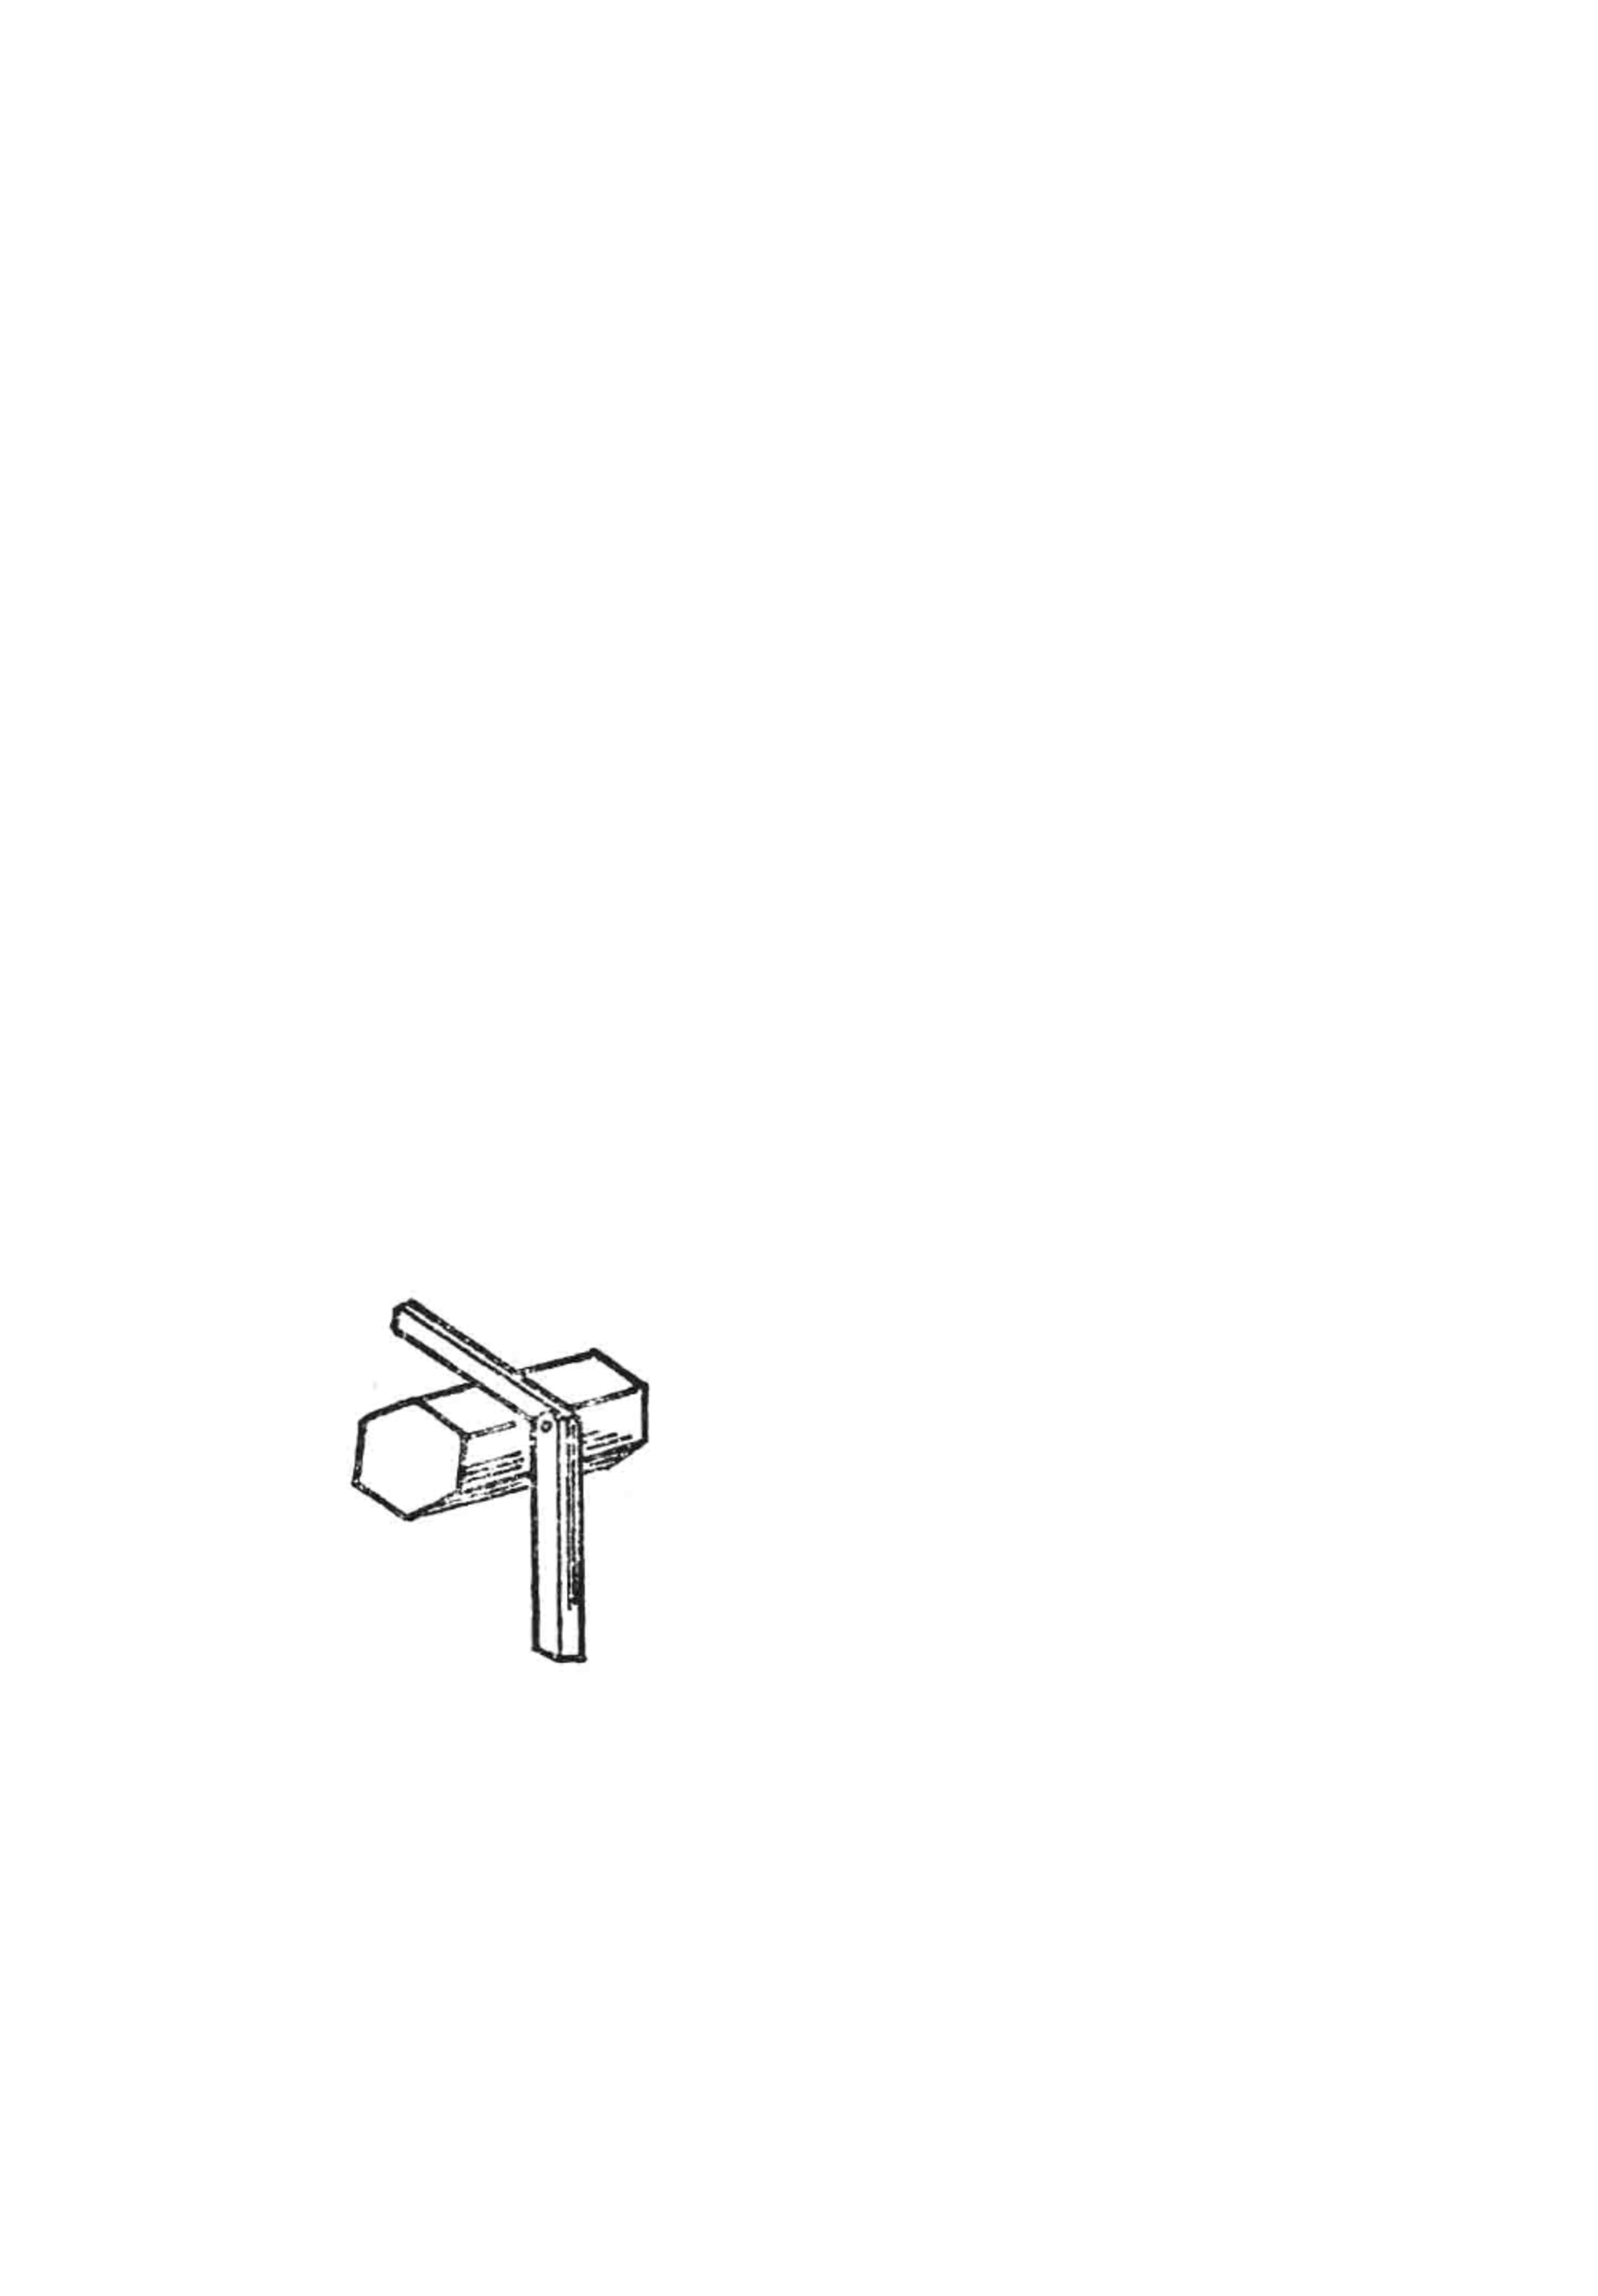
\includegraphics[scale=.4]{fig/1-61.pdf}
\captionof{figure}{}
\end{minipage}
\hfill
\begin{minipage}{.45\textwidth}
\centering
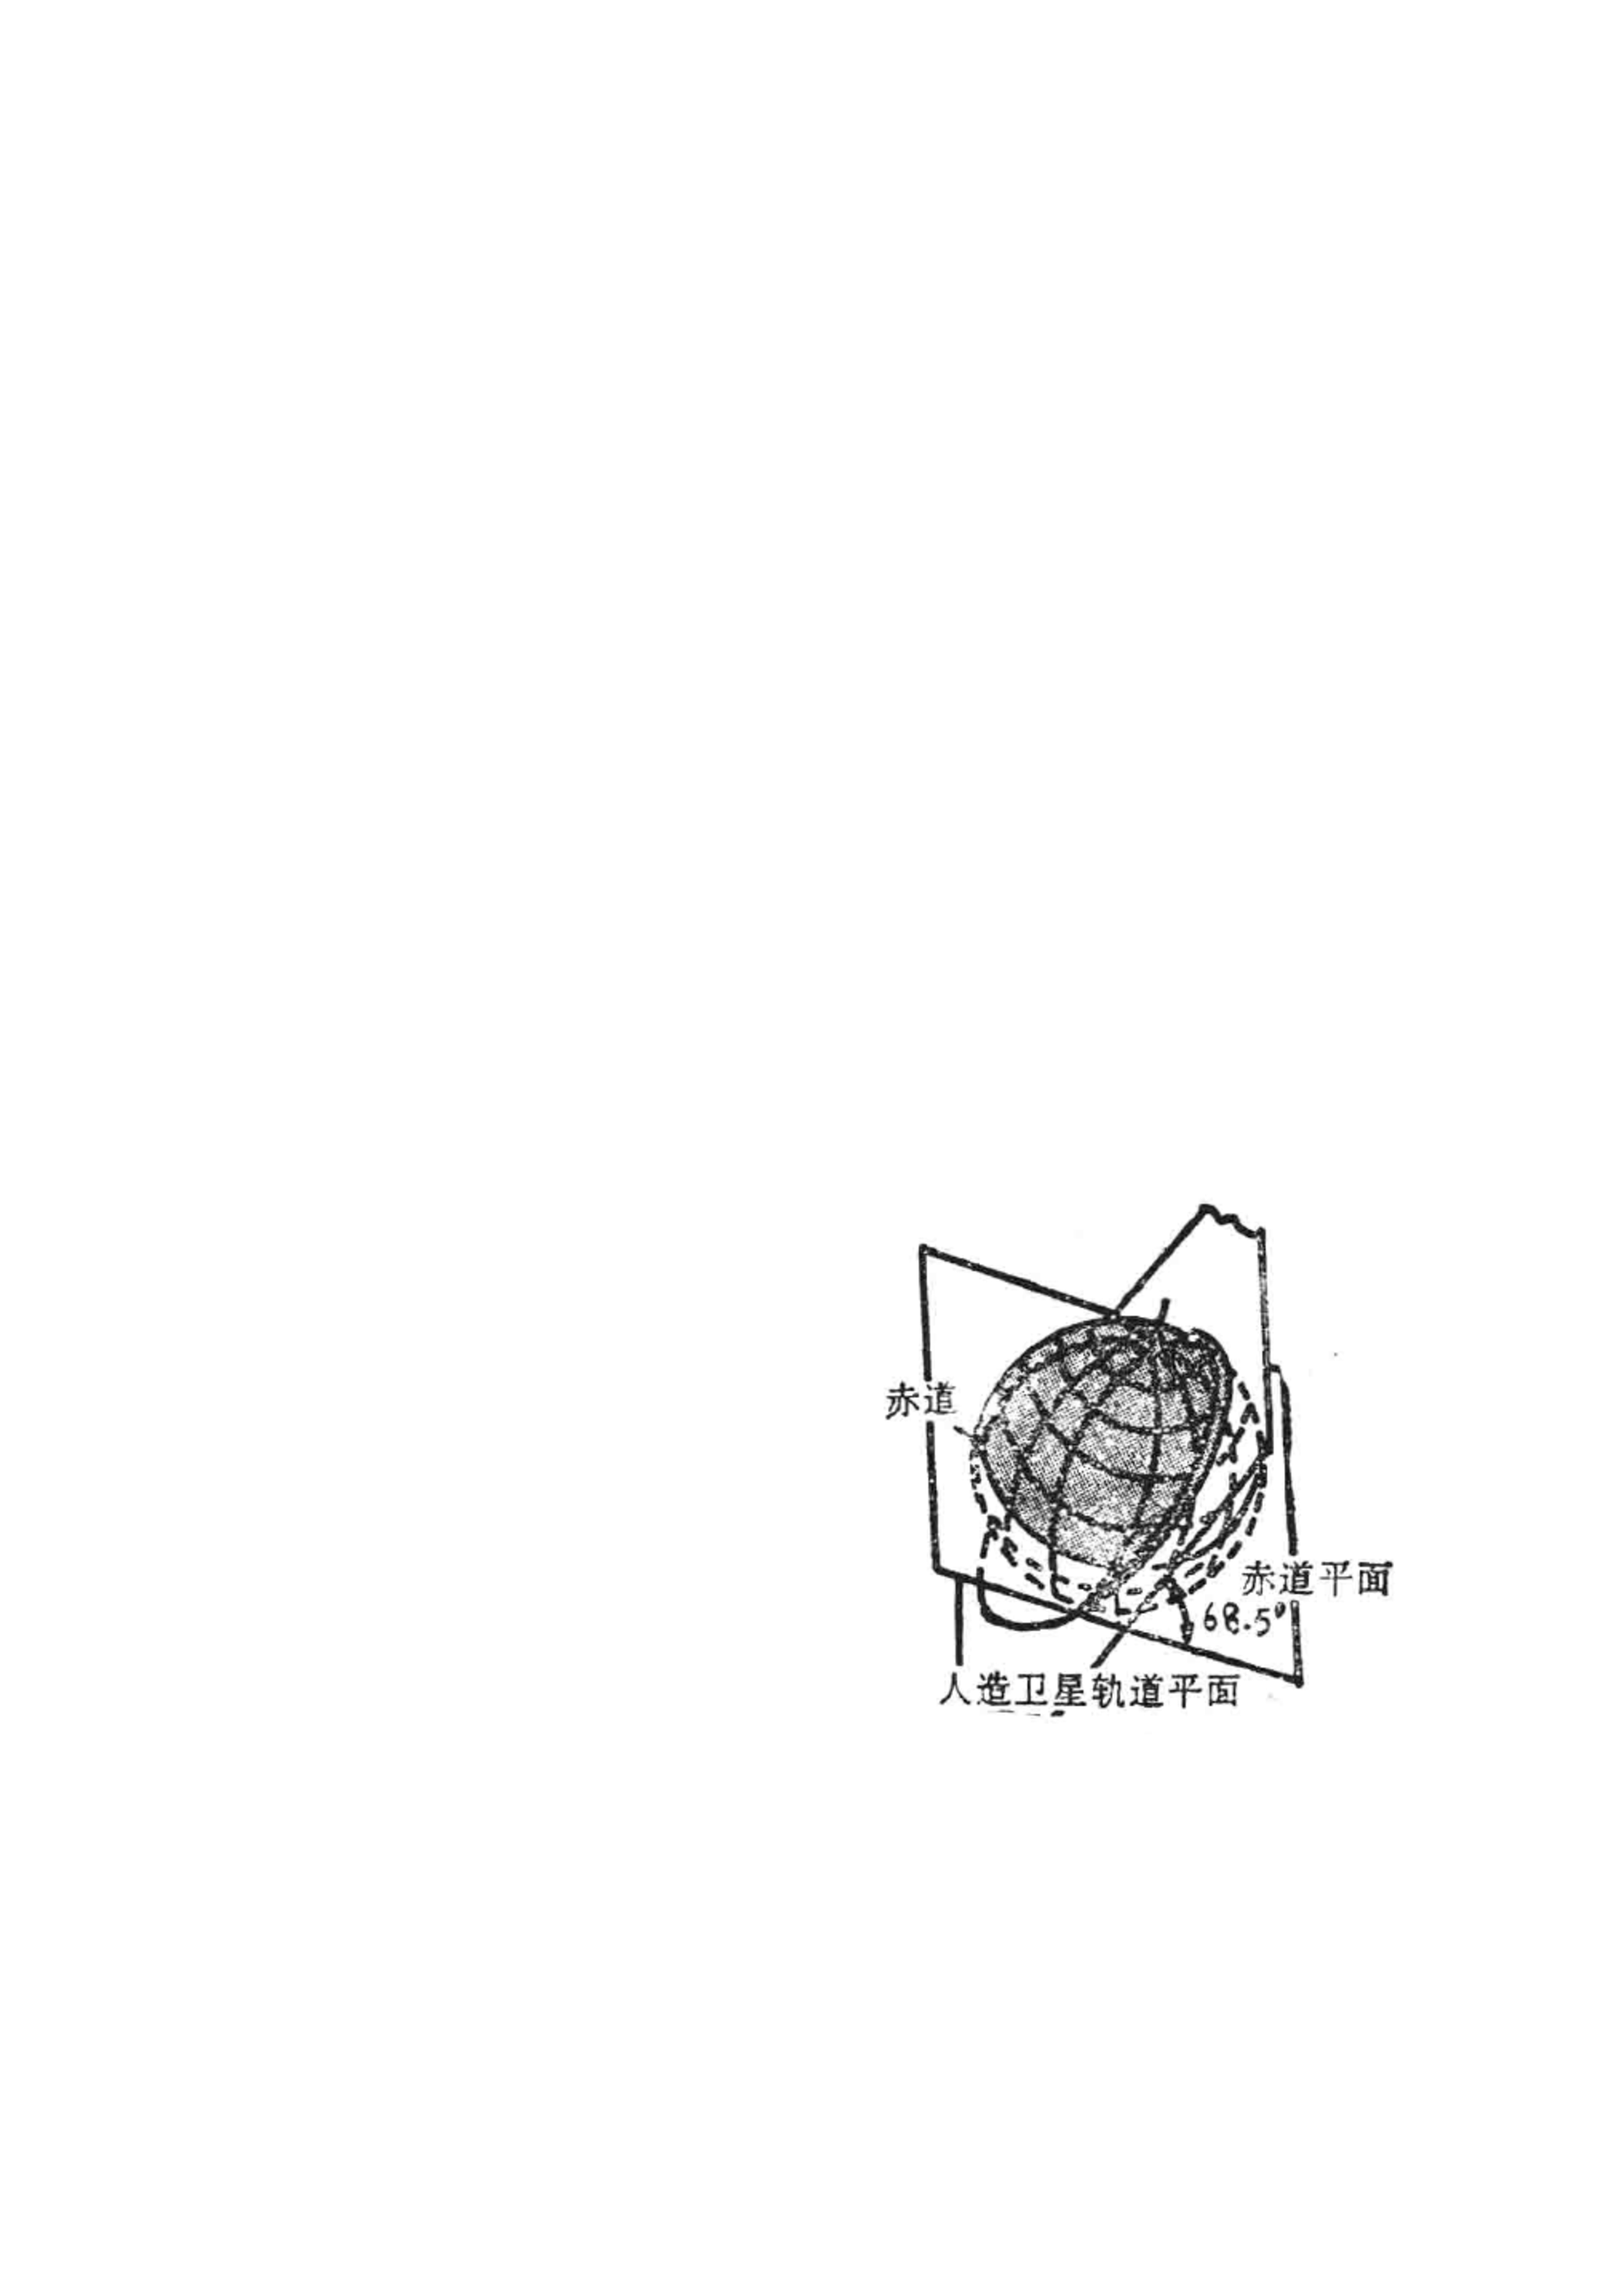
\includegraphics[scale=.4]{fig/1-62.pdf}
\captionof{figure}{}
\end{minipage}


\begin{example}
有一山坡的倾斜度（坡面与水平面所成的二面角的度数）是$60^{\circ}$．山坡上有一直路$CD$，它和斜坡底线$AB$成$30^{\circ}$角．沿这条直路行走100米，问升高了多少？
\end{example}

\begin{solution}
如图1.63，设$CD$是与斜坡底线$AB$成$30^{\circ}$角的直路，$CD=100$米．

    自$D$作垂直于地面的垂线段$DH$，设垂足是$H$，则线段
    $DH$的长就是所求的高度.

\noindent
\begin{minipage}{.58\textwidth}\CTEXindent
在平面$DCB$内过$D$作$DG\bot AB$于$G$，连$HG$，由三垂线逆定理，$HG\bot AB$，则$\angle DGH$就是坡面与地面所成二面角的平面角，
    
$\therefore\quad \angle DGH=60^{\circ}$，由此得：
\[\begin{split}
  DH&=DG\cdot \sin60^{\circ}\\
    &=CD\cdot \sin30^{\circ}\cdot \sin60^{\circ}\\
    &=25\sqrt{3}\; \text{（米）}．  
\end{split}\]
\end{minipage}
\hfill
\begin{minipage}{.4\textwidth}
\centering

\includegraphics[scale=.4]{FIG/1-63.PDF}
\captionof{figure}{}
\end{minipage}

\textbf{答：}沿这条直路前进100米，升高$25\sqrt{3}$米.
\end{solution}
    
\begin{example}
    如图1.64，自二面角$P-\ell-Q$的棱上一点$A$在平面$P$内引射线$AB$，和棱成$45^{\circ}$角，若$AB$和另一面$Q$成$30^{\circ}$角，求二面角$P-\ell-Q$的度数.
\end{example}

\begin{solution}
自射线$AB$上一点$B$向平面$Q$引垂线$BH$，$H$为垂足，连$HA$，则$\angle BAH$为$AB$与平面$Q$所成的角.

$\therefore\quad \angle BAH=30^{\circ}$. 

设$BH$长为$a$，则$AB=2a$, $AH=\sqrt{3}a$.

自$H$点向棱$\ell$作垂线$HC$，设$C$为垂足，由三垂线定理，$BC\bot AC$

$\therefore\quad \angle BCH$为二面角$P-\ell-Q$的平面角.

\noindent
\begin{minipage}{.58\textwidth}\CTEXindent
    在${\rm Rt}\triangle ABC$中，$\angle BAC=45^{\circ}$, $AB=2a$,

    $\therefore\quad AC=\sqrt{2}a$.
    
    在${\rm Rt}\triangle AHC$中，$AH=\sqrt{3}a$, $AC=\sqrt{2}a$
    
    $\therefore\quad HC=a$.
    
    在${\rm Rt}\triangle BHC$中，$HC=a$, $BH=a$,
    
    $\therefore\quad \angle BCH=45^{\circ}$
    
\end{minipage}
\hfill
\begin{minipage}{.4\textwidth}
\centering
\begin{tikzpicture}
    \tkzDefPoints{0/0/a, 3/0/b, 1.5/1.5/c, -1.5/1.5/d, -1.15/3.25/e}
    \tkzDefPointBy[translation = from a to e](b) \tkzGetPoint{f}
    \tkzDrawPolygon(a,b,c,f,e,d)
    
    \tkzDefPoints{0.5/1.5/C, -1/1.5/A}
    \tkzDefPointBy[translation = from d to e](C) \tkzGetPoint{C1}
    \tkzDefPointBy[translation = from d to a](C) \tkzGetPoint{C2}
    \tkzDefPointWith[linear, K=.8](C,C1) \tkzGetPoint{B}
    \tkzDefPointWith[linear, K=.5](C,C2)\tkzGetPoint{H}
    
    \tkzDrawPolygon[thick](A,H,B)
    \tkzDrawSegments[thick](B,C C,H c,d) 
    \tkzLabelPoints[below](A,H)
    \tkzLabelPoints[above left](C)
    \tkzLabelPoints[left](B)
    \node at (d)[above right]{$\ell$};
    \tkzLabelAngle[pos=.5](c,b,a){$Q$} 
    \tkzLabelAngle[pos=.4](e,f,c){$P$} 
    
    \end{tikzpicture}
\captionof{figure}{}
\end{minipage}

\textbf{答：}二面角$P-\ell-Q$的度数是$45^{\circ}$.


\end{solution}

\begin{example}
        如图1.65，已知二面角$P-\ell-Q$的度数为$120^{\circ}$，$A,B\in\ell$, $AC\subset P$，且$AC\bot AB$, $AC=4$; $BD\subset Q$, $BD\bot AB$, $BD=2$又$AB=6$. 求：$CD$的长.
    \end{example}

 \begin{analyze}
    欲求$CD$，需将问题转化为平面几何的计算题，再运用解三角形的方法来解决.
    
    由于已知二面角$P-AB-Q$的度数，又知$AC\bot \ell$于$A$，所以可以$A$为顶点、$AC$为一边作这个二面角的平面角.
    \end{analyze}


\begin{solution}
        在平面$Q$内作$AE\paraeq BD$，连结$DE$、$CE$，则四边形$ABDE$是平行四边形.

\noindent
\begin{minipage}{.53\textwidth}\CTEXindent
$\therefore\quad DE=AB=6$，$AE=BD=2$.

$\because\quad BD\bot AB$

$\therefore\quad AE\bot AB$

又$\because\quad AC\bot AB$,

$\therefore\quad \angle EAC$是二面角$P-\ell-Q$的平面角，

$\therefore\quad\angle CAE=120^{\circ}$.

$\because\quad AB\bot $平面$CAE$, $DE\parallel AB$,

$\therefore\quad DE\bot EC$.
\end{minipage}
\hfill
\begin{minipage}{.45\textwidth}
\centering
\begin{tikzpicture}[scale=.75]
\tkzDefPoints{0/0/b, -1.5/2.5/a, 3/0/c, 6/3/c'}
\foreach \x in {a,b}
 {
     \tkzDefPointBy[translation = from c to c'](\x) \tkzGetPoint{\x'}
 }
 \tkzDrawPolygon[](a,b,c,c',b',a')
 \tkzDrawSegments[](b,b') 

 \tkzDefPointWith[linear, K=.8](b,b') \tkzGetPoint{A}
 \tkzDefPointWith[linear, K=.3](b,b')\tkzGetPoint{B}

 \foreach \x in {A,B}
 {
     \tkzDefPointBy[translation = from b to c](\x) \tkzGetPoint{\x'}
 }
 \tkzDefPointWith[linear, K=.6](A,A') \tkzGetPoint{E}
 \tkzDefPointWith[linear, K=.6](B,B') \tkzGetPoint{D}

 \tkzDefPointBy[translation = from b to a](A) \tkzGetPoint{A''}
 \tkzDefPointWith[linear, K=.8](A,A'') \tkzGetPoint{C}
\tkzDrawSegments[thick](B,D D,E E,A C,A C,E C,D) 
\tkzLabelPoints[right](D,E)
\tkzLabelPoints[above](A)
\tkzLabelPoints[left](B,C)
\node at (b)[above]{$\ell$};
\tkzLabelAngle[pos=.6](b',c',c){$Q$} 
\tkzLabelAngle[pos=.6](a,a',b'){$P$} 
\end{tikzpicture}
\captionof{figure}{}
\end{minipage}

\[\begin{split}
\because\quad CD^2&=DE^2+CE^2\\
&=AB^2+\left(AE^2+AC^2-2AC\cdot AE\cos120^{\circ}\right)\\
&=36+4+16+8=64
\end{split}\]

$\therefore\quad CD=8$

还可以这样想：

过$C$点作$CF\bot $平面$Q$于$F$，过$D$点作$DE\parallel AB$，交直线$FA$于$E$，连结$DF$（请读者自己作图）.

$\because\quad CF\bot $平面$Q$于$F$，$AB\bot AC$,

$\therefore\quad AB\bot EF$（三垂线定理的逆定理），

$\therefore\quad \angle CAE$是二面角$P-\ell-Q$的平面角，

$\therefore\quad \angle CAF=180^{\circ}-\angle CAE=60^{\circ}$.

在${\rm Rt}\triangle CAF$中，得
\[CF=AC\sin60^{\circ}=2\sqrt{3},\quad AF=2\]

在${\rm Rt}\triangle FED$中，得
\[DF^2=EF^2+DE^2=16+36=52\]

在${\rm Rt}\triangle CFD$中，得
\[CD^2=CF^2+FD^2=12+52=64\]

$\therefore\quad CD=8$.
\end{solution}

\subsection*{1.14 练习}
\begin{enumerate}
\item 例1.22中“过$D$作$DG\bot AB$于$G$，连$HG$”换为“过$H$在
平面$ABH$内作$HG\bot AB$于$G$，连$DG$”所得的$\angle DGH$还是二面角$D-AB-H$的平面角吗？
\item 一个平面垂直于二面角的棱，它和二面角的两个面的交线所成的角就是二面角的平面角，为什么？
\item 下列各题中，用适当的方法作出二面角的平面角。
\begin{enumerate}[(1)]
\item 拿一张锐角三角形纸片$ABC$，以它的高$AD$为折痕，折成一个二面角，找出二面角$B-AD-C$的平面角.
\item 在$30^{\circ}$的二面角的一个面内有一个点，它到另一个面的距离是10cm，求它到棱的距离（提示：用三垂线定理作出二面角的平面角）.
\item 自二面角内一点分别向两个面引垂线。求证：它们所成的角与二面角的平面角互补（提示：过这两条垂线的平面与二面角的棱垂直，它与二面角的两个面的交线所成的角就是二面角的平面角）.
\end{enumerate}

\item 总结作出二面角的平面角的方法。
\end{enumerate}

\section{两个平面垂直的判定}
两个相交平面的位置关系，可由它们所成的二面角的大小来描述，现在我们来研究两个相交平面的特殊情况——垂直.

\begin{thm}
 {定义} 两个平面相交，如果所成的二面角是直二面角，就说这两个平面互相垂直. 若平面$\alpha$和$\beta$互相垂直，记作
$\alpha\bot\beta$.   
\end{thm}

两个互相垂直的平面，如果有一个是水平平面，则把直
立平面的一边画成和水平平面的某一边垂直．如图1.66．

\begin{figure}[htp]
    \centering
\begin{tikzpicture}
\begin{scope}
\tkzDefPoints{0/0/A, 3/0/B, 4/1/C, 0.5/.5/E, .5/2/F}
\tkzDefPointBy[translation = from B to C](A) \tkzGetPoint{D}
\foreach \x in {E,F}
{
    \tkzDefPointBy[translation = from A to B](\x) \tkzGetPoint{\x'}
}
\tkzDrawPolygon(E,F,F',E')
\tkzDrawPolygon(A,B,E',E)
\tkzInterLL(C,D)(E',F')  \tkzGetPoint{tmp}
\tkzInterLL(A,D)(E,F)  \tkzGetPoint{tmp1}
\tkzDrawSegments[dashed](tmp,D) 
\tkzDrawSegments[thick](tmp,C  C,E') 
\tkzDrawSegments[dashed](tmp1,D) 
\tkzLabelAngle[pos=.6](B,A,D){$\alpha$} 
\tkzLabelAngle[pos=.4](E,F,F'){$\beta$} 
\node at (2,-.5){(1)};
\end{scope}
\begin{scope}[xshift=5cm] 
\tkzDefPoints{0/0/A, 3/0/B, 4/1/C, 1.5/0/E, 1.5/1.5/F}
\tkzDefPointBy[translation = from B to C](A) \tkzGetPoint{D}
\foreach \x in {E,F}
{
    \tkzDefPointBy[translation = from B to C](\x) \tkzGetPoint{\x'}
}
\tkzDrawPolygon(E,F,F',E')
\tkzDrawPolygon(E,B,C,E')
\tkzInterLL(C,D)(E,F)  \tkzGetPoint{tmp}
\tkzDrawSegments[dashed](E',tmp) 
\tkzDrawSegments[](tmp,D  D,A A,E) 
\tkzLabelAngle[pos=.6](B,A,D){$\alpha$} 
\tkzLabelAngle[pos=.4](F,F',E'){$\beta$} 
    \node at (2,-.5){(2)};
\end{scope}
\end{tikzpicture}

    \caption{}
\end{figure}

除了定义以外，还可怎样判定两个平面垂直呢？我们知道，判定面面关系，往往利用线面关系.

\begin{thm}
  {两个平面垂直的判定定理} 如果一个平面经过另一个平面的一条垂线，那么这两个平面互相垂直.  
\end{thm}

\begin{example}
    已知：$AB\bot\beta$, $AB\subset \alpha$（如图1.67）．
    求证：$\alpha\bot\beta$.
\end{example}

\begin{proof}
设$AB\cap \beta = B$, $\alpha\cap \beta=CD$，则$B\in CD$.

\noindent
\begin{minipage}{.6\textwidth}
\CTEXindent
    $\because\quad AB\bot\beta,\quad CD\subset \beta$,

    $\therefore\quad AB\bot CD$. 
    
    在平面$\beta$ 内过点$B$作直线$BE\bot CD$，则$\angle ABE$是二面角$\alpha-CD-\beta$ 的平面角.
    
    $\because\quad AB\bot \beta$ 
    
    $\therefore\quad AB\bot BE, \quad \angle ABE=90^{\circ}$. 
    即二面角$\alpha-CD-\beta$ 是直二面角.
    
    $\therefore\quad \alpha\bot \beta$.
\end{minipage}
\hfill
\begin{minipage}{.38\textwidth}
\centering
\begin{tikzpicture}[]
    \tkzDefPoints{0/0/A, 3/0/B, 4/1/C, 1.5/0/E, 1.5/1.5/F}
    \tkzDefPointBy[translation = from B to C](A) \tkzGetPoint{D}
    \foreach \x in {E,F}
    {
        \tkzDefPointBy[translation = from B to C](\x) \tkzGetPoint{\x'}
    }
    \tkzDrawPolygon(E,F,F',E')
    \tkzDrawPolygon(E,B,C,E')
    \tkzInterLL(C,D)(E,F)  \tkzGetPoint{tmp}
    \tkzDrawSegments[dashed](E',tmp) 
    \tkzDrawSegments[](tmp,D  D,A A,E) 
    \tkzLabelAngle[pos=.6](B,A,D){$\beta$} 
    \tkzLabelAngle[pos=.4](F,F',E'){$\alpha$} 
    \tkzDefMidPoint(E,E')\tkzGetPoint{B}
    \draw[thick](B)node[below]{$B$}--+(0,1.2)node[right]{$A$};
    \draw[thick](B)--+(1.25,0)node[above]{$E$};
    \node at (E)[below]{$C$};
    \node at (E')[above right]{$D$};
\end{tikzpicture}
\captionof{figure}{}
\end{minipage}
\end{proof}

\begin{example}
    如图1.68，已知$P$是平面$\alpha$外一点，$PA\bot \alpha$于$A$, $BC\subset a$，$PC\bot BC$于$C$，求证：平面$PBC\bot $平面$PAC$.
\end{example}

\begin{analyze}
   欲证平面$PBC$上平面$PAC$，只需证其中一平面经过另一平面的垂线.
\end{analyze}

\noindent
\begin{minipage}{.45\textwidth}\CTEXindent
\begin{proof}
$\because\quad PA\bot $平面$\alpha$，$BC\subset\alpha$

$\therefore\quad PA\bot BC$，又$PC\bot BC$.

$\because\quad PA\cap PC=P$,

$\therefore\quad BC\bot$平面$PAC$.

又$\because\quad BC\subset $平面$PBC$，

$\therefore\quad $平面$PBC\bot $平面$PAC$.
\end{proof}
\end{minipage}
\hfill
\begin{minipage}{.5\textwidth}
\centering
\begin{tikzpicture}[scale=1.3]
\tkzDefPoints{0/0/a, 3/0/b, 4/1/c, 1/1/d, 1.5/.6/A, 1.5/2/P, 2.2/.3/C, 2.7/.8/B}
\tkzDrawPolygon[thick](P,A,C,B)
\tkzDrawPolygon(a,b,c,d)
\tkzDrawSegments[thick](P,C) 
\tkzLabelPoints[below right](C)
\tkzLabelPoints[above](P)
\tkzLabelAngle[pos=.4](b,a,d){$\alpha$} 
\tkzLabelPoints[left](A)
\tkzLabelPoints[right](B)

\end{tikzpicture}
\captionof{figure}{}
\end{minipage}

\subsection*{1.15 练习}
\begin{enumerate}
\item 画互相垂直的两个平面、两两垂直的三个平面．

\noindent
\begin{minipage}{.6\textwidth}
    \item 如图，检查工件的相邻两个平面是否垂直时，只要用曲尺的一边紧靠在工件的一个面上，另一边在工件的另一个面上转动一下，观察尺边是否和这个面密合就可以了。为什么？如果不转动呢？

\end{minipage}
\hfill
\begin{minipage}{.35\textwidth}
\centering
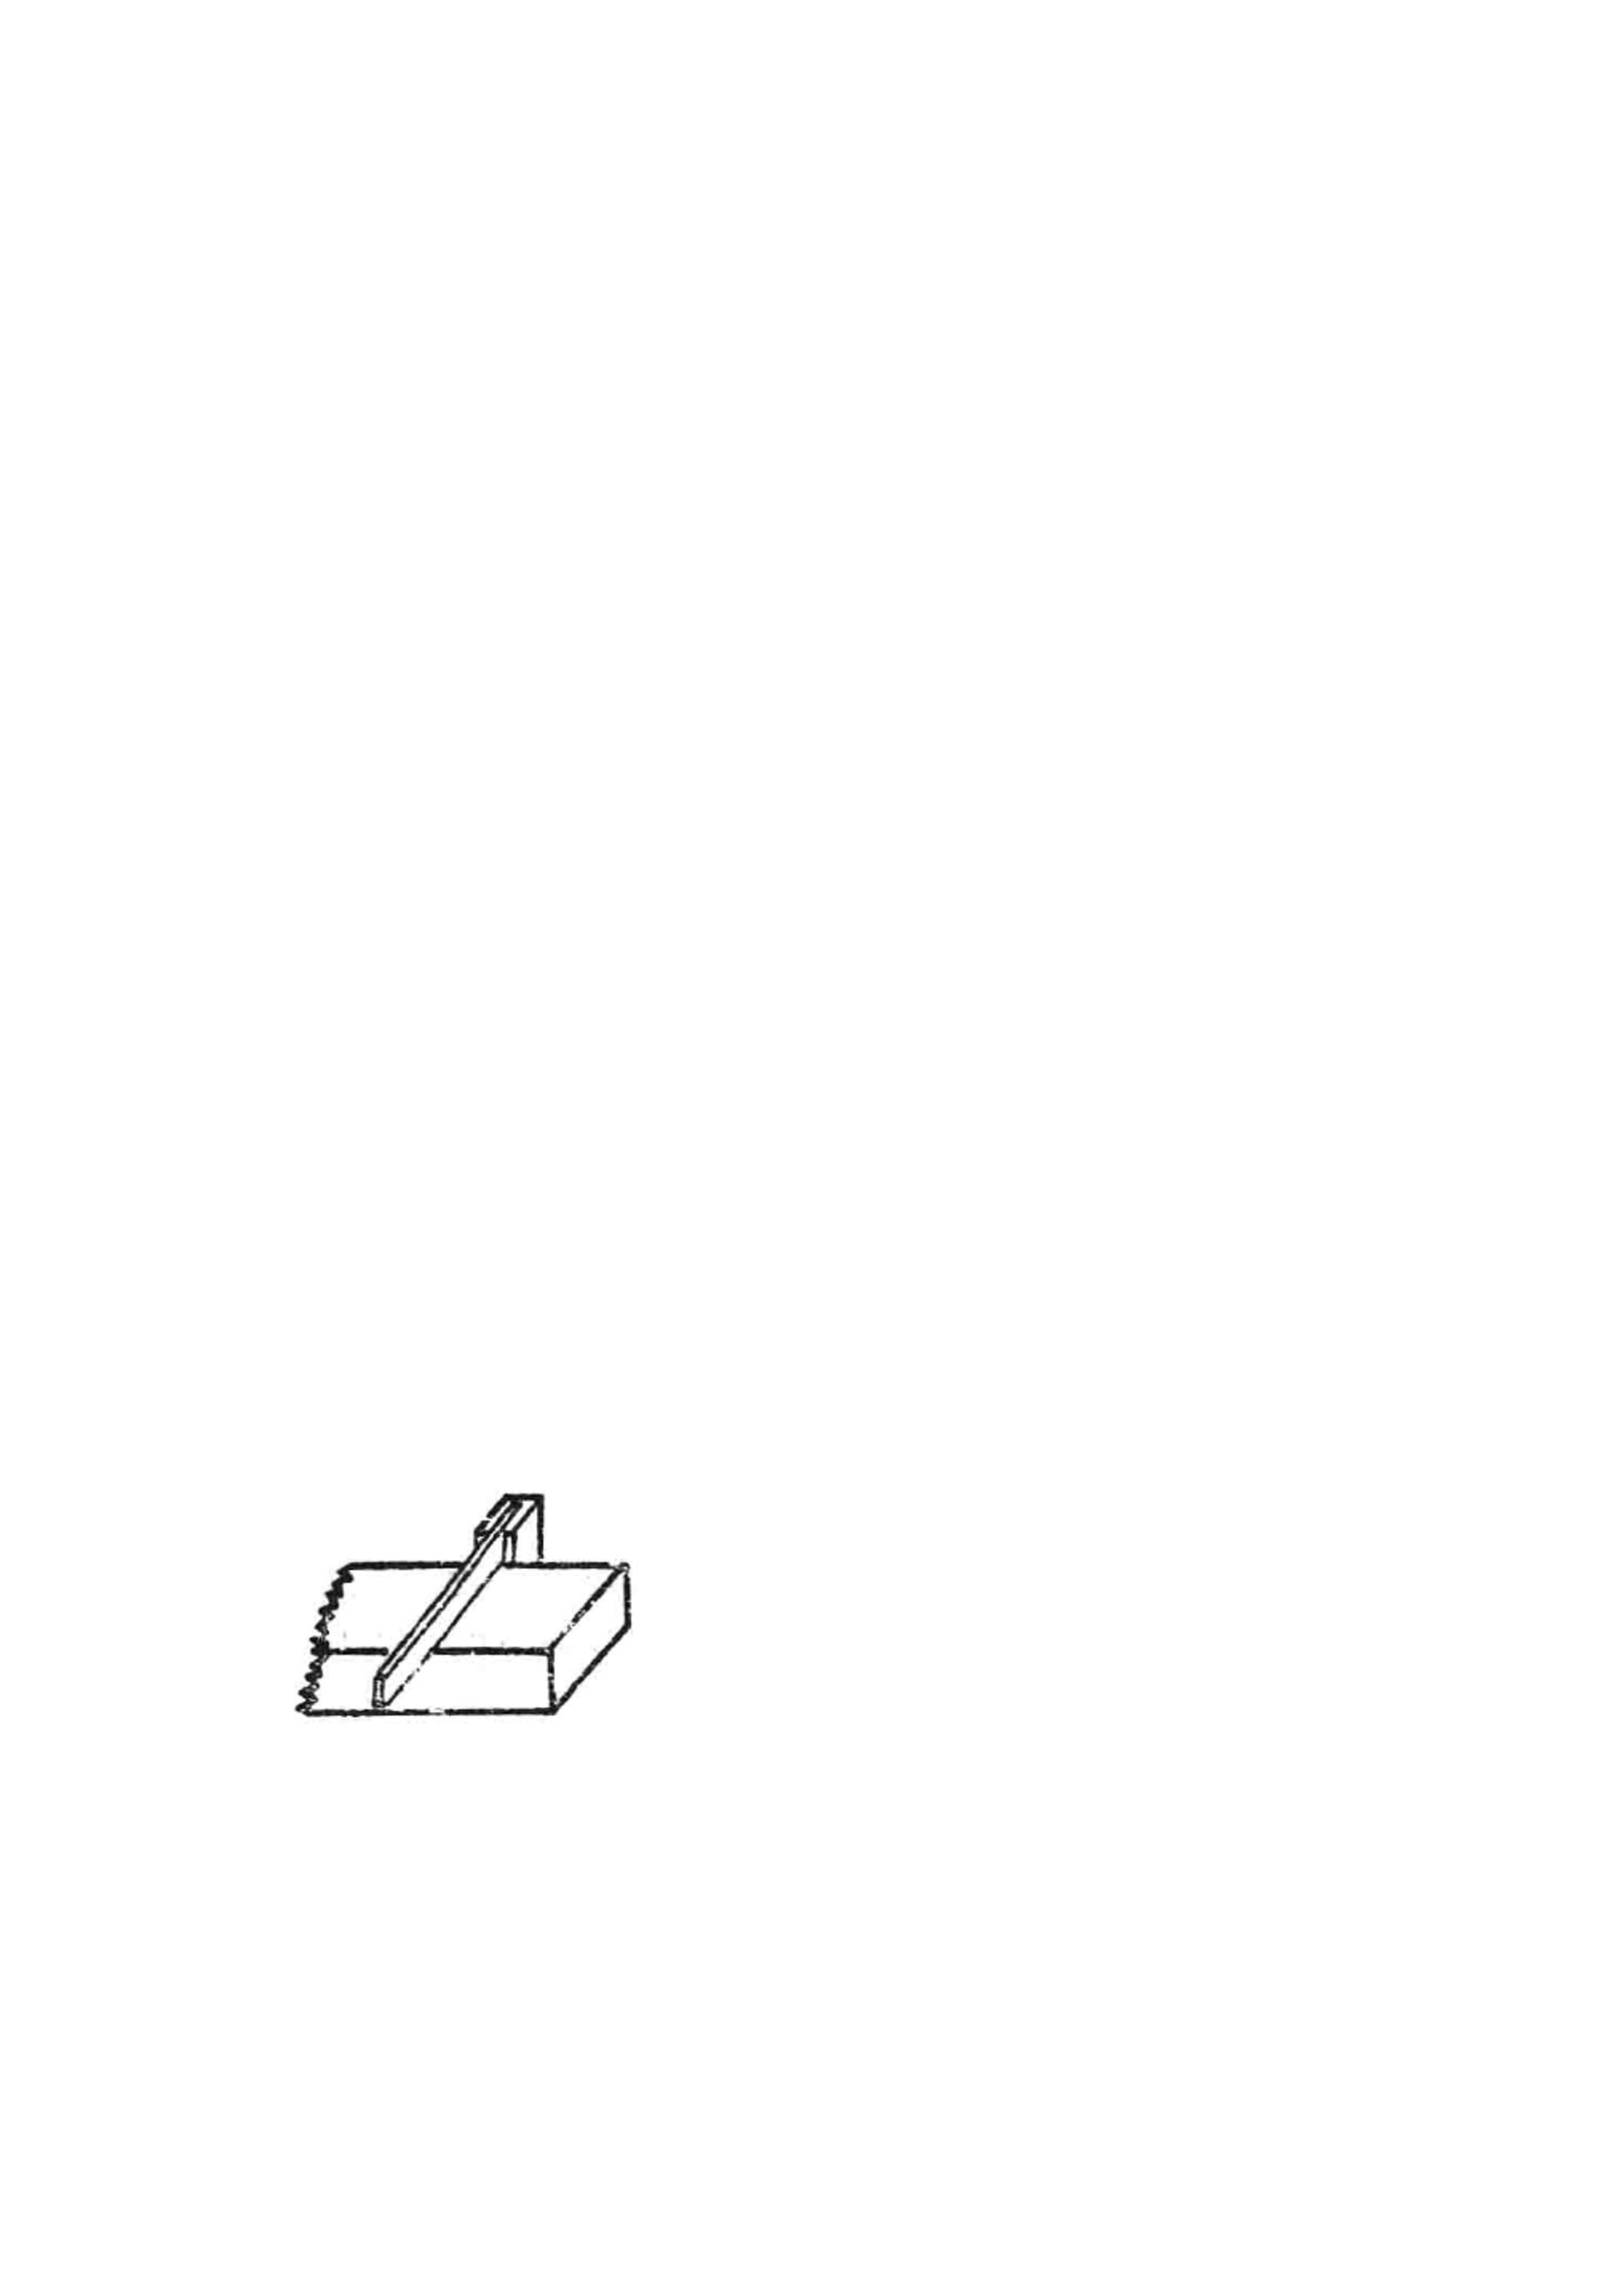
\includegraphics[scale=.45]{fig/1-ex2.pdf}
\captionof*{figure}{第2题}
\end{minipage}

    \item 建筑工人在砌墙时，依据直线和平面垂直的判定定理常用一端系有铅锤的线来检查所砌的墙面是否和地面垂
    直，应怎样检查？
\end{enumerate}

\section{两个平面垂直的性质}
由两个平面垂直可以推出什么样的“线面”关系和“线线”关系呢？


\noindent
\begin{minipage}{.6\textwidth}
\begin{thm}
  {两个平面垂直的性质定理1} 如果两个平面垂直，那么在一个平面内垂直于它们交线的直线垂直于另一个平面.  
\end{thm}

已知：如图1.69, $\alpha\bot\beta$, $\alpha\cap\beta =CD$, $AB\subset \alpha$, $AB\bot CD$.

求证：$AB\bot \beta$.
\end{minipage}
\hfill
\begin{minipage}{.38\textwidth}
\centering
\begin{tikzpicture}[]
    \tkzDefPoints{0/0/A, 3/0/B, 4/1/C, 1.5/0/E, 1.5/1.5/F}
    \tkzDefPointBy[translation = from B to C](A) \tkzGetPoint{D}
    \foreach \x in {E,F}
    {
        \tkzDefPointBy[translation = from B to C](\x) \tkzGetPoint{\x'}
    }
    \tkzDrawPolygon(E,F,F',E')
    \tkzDrawPolygon(E,B,C,E')
    \tkzInterLL(C,D)(E,F)  \tkzGetPoint{tmp}
    \tkzDrawSegments[dashed](E',tmp) 
    \tkzDrawSegments[](tmp,D  D,A A,E) 
    \tkzLabelAngle[pos=.6](B,A,D){$\beta$} 
    \tkzLabelAngle[pos=.4](F,F',E'){$\alpha$} 
    \tkzDefMidPoint(E,E')\tkzGetPoint{B}
    \draw[thick](B)node[below]{$B$}--+(0,1.2)node[right]{$A$};
    \draw[thick](B)--+(1.25,0)node[above]{$E$};
    \node at (E)[below]{$C$};
    \node at (E')[above right]{$D$};
\end{tikzpicture}
\captionof{figure}{}
\end{minipage}



\begin{proof}
设$AB\bot CD$于$B$，在平面$\beta$ 内，过$B$作$BE\bot CD$，则$\angle ABE$是二面角$\alpha-CD-\beta$ 的平面角.

$\because\quad \alpha\bot \beta$ 

$\therefore\quad AB\bot BE$

由已知$AB\bot CD$，而$CD\cap BE=B$,

$\therefore\quad AB\bot \beta$.
\end{proof}

\begin{thm}
    {两个平面垂直的性质定理2} 如果两个平面互相垂直，那么经过第一个平面内的一点垂直于第二个平面的直线，在第一个平面内.
\end{thm}

已知：$\alpha\bot\beta$, $A\in\alpha$, $AB\bot \beta$.

求证：$AB\subset \alpha$.

\begin{proof}
    如图1.70，设$\alpha\cap\beta =CD$. 在$\alpha$内，过点$A$作$AB'\bot CD$．根据定理1，$AB'\bot \beta$.
\begin{figure}[htp]
    \centering
\begin{tikzpicture}[scale=1.2]
\begin{scope}
\tkzDefPoints{0/0/A, 3/0/B, 4/1/C, 1.5/0/E, 1.5/1.5/F}
\tkzDefPointBy[translation = from B to C](A) \tkzGetPoint{D}
\foreach \x in {E,F}
{
    \tkzDefPointBy[translation = from B to C](\x) \tkzGetPoint{\x'}
}
\tkzDrawPolygon(E,F,F',E')
\tkzDrawPolygon(E,B,C,E')
\tkzInterLL(C,D)(E,F)  \tkzGetPoint{tmp}
% \tkzDrawSegments[dashed](E',tmp) 
\tkzDrawSegments[](tmp,D  D,A A,E) 
\tkzLabelAngle[pos=.6](B,A,D){$\beta$} 
\tkzLabelAngle[pos=.4](F,F',E'){$\alpha$} 
\tkzDefMidPoint(E,E')\tkzGetPoint{B}
\draw[thick](B)node[left]{$B'$}--+(0,1.2)node[right]{$A$}--+(.2,-.3)node[right]{$B$};

\node at (E)[below]{$C$};
\node at (E')[above right]{$D$};
\node at (1.5,-.75){甲};
\end{scope}

\begin{scope}[xshift=5cm]
\tkzDefPoints{0/0/A, 3/0/B, 4/1/C, 1.5/0/E, 1.5/1.5/F}
\tkzDefPointBy[translation = from B to C](A) \tkzGetPoint{D}
\foreach \x in {E,F}
{
    \tkzDefPointBy[translation = from B to C](\x) \tkzGetPoint{\x'}
}
\tkzDrawPolygon(E,F,F',E')
\tkzDrawPolygon(E,B,C,E')
\tkzInterLL(C,D)(E,F)  \tkzGetPoint{tmp}
% \tkzDrawSegments[dashed](E',tmp) 
\tkzDrawSegments[](tmp,D  D,A A,E) 
\tkzLabelAngle[pos=.6](B,A,D){$\beta$} 
\tkzLabelAngle[pos=.4](F,F',E'){$\alpha$} 
\tkzDefMidPoint(E,E')\tkzGetPoint{B}
\draw[thick](B)node[below]{$A$}--+(0,1.2)node[below left]{$B'$};
\draw[thick](B)--+(0.2,1.2)node[below right]{$B$};
\node at (E)[below]{$C$};
\node at (E')[above right]{$D$};
\node at (1.5,-.75){乙};

\end{scope}
\end{tikzpicture}
    \caption{}
\end{figure}

因为过一点只有一条直线与平面$\beta$ 垂直，所以$AB'$与直线$AB$是同一条直线.

$\because\quad AB'\subset \alpha$

$\therefore\quad AB\subset \alpha$
\end{proof}



\begin{example}
    已知$\alpha \bot \gamma$, $\beta\bot\gamma$, $\alpha\cap \beta=a$（如图1.71）. 
求证：$\alpha\bot \gamma$.
\end{example}

\noindent
\begin{minipage}{.6\textwidth}
    \CTEXindent
\begin{proof}
在$a$上任取一点$A$，过$A$作直线$a'\bot \gamma$.

$\because\quad \alpha \bot \gamma,\quad A\in a$

$\therefore\quad a'\subset \alpha$

同理$a'\subset \beta$

$\therefore\quad a'=\alpha\cap \beta$.

$\because\quad a'$和$a$重合而$a'\bot\gamma$

$\therefore\quad a\bot\gamma$.
\end{proof}
\end{minipage}
\hfill
\begin{minipage}{.35\textwidth}
\centering
\begin{tikzpicture}[]
    \tkzDefPoints{0/0/a, 3/0/b, 4/1.5/c, 1/1.5/d}

    \tkzDefPoints{1.2/.3/a1, 2.1/.8/b1, 3/.5/c1, 1.2/2/a11}
    \foreach \x in {b1,c1}
    {
        \tkzDefPointBy[translation = from a1 to a11](\x) \tkzGetPoint{\x1}
    }
    \tkzDrawPolygon(a1,b1,c1,c11,b11,a11)
    \tkzDrawSegments[thick](b1,b11) 
    \tkzDrawSegments[](a,b b,c d,a) 
    \tkzInterLL(c,d)(a1,a11)  \tkzGetPoint{tmp1}
    \tkzInterLL(c,d)(c1,c11)  \tkzGetPoint{tmp2}
    \tkzDrawSegments[](d,tmp1 c,tmp2) 
    \tkzLabelAngle[pos=.3](b11,c11,c1){$\beta$} 
    \tkzLabelAngle[pos=.3](a1,a11,b11){$\alpha$} 
    \tkzLabelAngle[pos=.4](b,a,d){$\gamma$} 
    \node at (b1)[above left]{$a'$};
    \node at (b1)[above right]{$a$};
    \tkzDefPointWith[linear, K=.2](b11,b1) \tkzGetPoint{A}
    \tkzDrawPoints(A)  \tkzLabelPoints[right](A)
\end{tikzpicture}
\captionof{figure}{}
\end{minipage}



\begin{example}
如图1.72，$D$为等边$\triangle ABC$所在平面外一点，已知$AB=a$, $DC=\frac{1}{2}a$, $DA=DB=\frac{\sqrt{3}}{2}a$. 求$D$点到平面$ABC$的距离.
\end{example}


\begin{solution}
取$AB$的中点$E$，连$DE$、$CE$.

\noindent
\begin{minipage}{.5\textwidth}\CTEXindent
$\because\quad    DA=DB$

$\therefore\quad DE\bot AB$

$\because\quad CB=CA$

$\therefore\quad CE\bot AB$，而$CE\cap DE=E$

$\therefore\quad AB\bot$平面$DEC$

$\therefore\quad $平面$DEC\bot $平面$ABC$.

\end{minipage}
\hfill
\begin{minipage}{.45\textwidth}
\centering
\begin{tikzpicture}[scale=1.1]
    \tkzDefPoints{0/0/A, 3/0/C, 2.5/-1/B, 1.8/1.2/D, 1.8/-.3/H}
    \tkzDrawPolygon[thick](A,B,C,D)
    \tkzInterLL(C,H)(A,B)  \tkzGetPoint{E}
    \tkzDrawSegments[thick](D,E D,B) 
    \tkzDrawSegments[dashed](D,H C,E A,C) 
    \tkzLabelPoints[below](E,B,H) 
    \tkzLabelPoints[right](C) 
    \tkzLabelPoints[left](A) 
    \tkzLabelPoints[above](D) 
\end{tikzpicture}
\captionof{figure}{}
\end{minipage}

在平面$DEC$内过$D$作$DH\bot EC$于$H$，则$DH\bot $平面$ABC$.

在${\rm Rt}\triangle DAE$中

$\because\quad AD=\frac{\sqrt{3}}{2}a,\quad AE=\frac{1}{2}AB=\frac{1}{2}a,\quad AE\bot ED$

$\therefore\quad DE=\frac{\sqrt{2}}{2}a$

在等边$\triangle ABC$中

$\because\quad AB=a,\quad CE\bot AB$

$\therefore\quad CE=\frac{\sqrt{3}}{2}a$

在$\triangle DCE$中

$\because\quad DC=\frac{1}{2}a,\quad CE=\frac{\sqrt{3}}{2}a,\quad DE=\frac{\sqrt{2}}{2}a$

$\therefore\quad \angle CDE=90^{\circ}$

$\because\quad DH=\frac{DE\cdot DC}{CE}=\frac{\frac{\sqrt{2}}{2}a\cdot \frac{1}{2}a}{\frac{\sqrt{3}}{2}a}=\frac{\sqrt{6}}{6}a$

$\therefore\quad D$点到平面$ABC$的距离是$\frac{\sqrt{6}}{6}a$.
\end{solution}



\begin{example}
    已知两条异面直线$a$、$b$所成的角是$\theta$，$AA'$是它们的公垂线段，且长为$d$，若$E\in a$, $F\in b$，且$A'E=m$, $AF=n$，求$EF$.
\end{example}

\begin{solution}
过$A$作直线$c\parallel a$, 因为$a$、$b$所成的角是$\theta$. 所以，$b$、$c$所成的锐角或直角等于$\theta$．

在$a$、$c$确定的平面β内，过$E$点作$EG\bot c$于$G$，则$EG$垂直$b$、$c$确定的平面$\alpha$

$\therefore\quad EG\bot GF$，且$AG\paraeq A'E$,

$\therefore\quad AG=m$.

\begin{enumerate}[(1)]
\item 若$\angle GAF=\theta$，如图1.73，
则$GF^2=m^2+n^2-2mn\cos\theta$.

$\because\quad EG\bot FG$

$\therefore\quad EF^2=GF^2+EG^2$.

$\therefore\quad EF=\sqrt{GF^2+EG^2}=\sqrt{d^2+m^2+n^2-2mn\cos\theta}$.

\noindent
\begin{minipage}{.45\textwidth}
\centering
\begin{tikzpicture}[]
    \tkzDefPoints{0/0/a, 4/0/b, 5/1.5/c, 1/1.5/d}
    \tkzDrawPolygon[](a,b,c,d)
    \tkzDefPoints{1.5/1/A, 3.5/1/G, 1.5/3/A', 3.5/3/E, 2.5/.5/F}
    \tkzDrawLines[add= 0 and .2, thick](A,G) 
    \tkzDrawLines[add= .2 and .4](A,F) 
    \tkzDrawLines[add= .4 and .4, thick](A',E) 
    \tkzDrawSegments[thick](A,A' E,G F,G E,F) 
    \tkzLabelPoints[below](A,F,G) 
    \tkzLabelPoints[above](A',E) 
    \draw(A')--node[above]{$m$}(E);
    \draw(A)--node[above]{$m$}(G);
    \draw(A)--node[below]{$n$}(F);
    \node at (3,.2){$b$};
    \node at (4,1){$c$};
    \node at (4.5,3){$a$};
    \tkzMarkAngles[mark=none, size=.5](F,A,G) 
    \tkzLabelAngle[pos=.7](F,A,G){$\theta$} 
\end{tikzpicture}
\captionof{figure}{}
\end{minipage}
\hfill
\begin{minipage}{.45\textwidth}
\centering
\begin{tikzpicture}[]
    \tkzDefPoints{0/-.2/a, 4/-.2/b, 5/1.75/c, 1/1.75/d}
    \tkzDrawPolygon[](a,b,c,d)
    \tkzDefPoints{2.5/.3/A, 3.5/.3/G, 2.5/3/A', 3.5/3/E, 1.25/1.35/F}
    \tkzDrawLines[add= 1.7 and 0, thick](A,G) 
    \tkzDrawLines[add= .4 and .1](A,F) 
    \tkzDrawLines[add= .7 and .7, thick](A',E) 
    \tkzDrawSegments[thick](A,A' E,G F,G E,F) 
    \tkzLabelPoints[below](A,F) 
    \tkzLabelPoints[right](G) 
    \tkzLabelPoints[above](A',E) 
    \draw(A')--node[above]{$m$}(E);
    \draw(A)--node[above]{$m$}(G);
    \draw(A)--node[below]{$n$}(F);
    \node at (1,1.4){$b$};
    \node at (.5,.3){$c$};
    \node at (4.5,3){$a$};
    
    \tkzDefPointWith[linear, K=1.5](F,A) \tkzGetPoint{A''}
    \tkzLabelAngle[pos=.6](A'',A,G){$\theta$} 
    \tkzMarkAngles[mark=none, size=.4](A'',A,G) 
\end{tikzpicture}
\captionof{figure}{}
\end{minipage}

\item 若$\angle GAF=180^{\circ}-\theta$．如图1.74．则
\[\begin{split}
    GF^2&=m^2+n^2-2mn\cos(180^{\circ}-\theta)\\
    &=m^2+n^2-2mn\cos\theta
\end{split}\]

$\therefore\quad EF=\sqrt{d^2+m^2+n^2-2mn\cos\theta}$.
\end{enumerate}

这就是异面直线上两点间的距离公式. 由式中可以看出，
当$m=0$，且$n=0$时，$EF$有最小值.
$$EF_{\min}=d$$

所以，两条异面直线的距离是分别在两条异面直线上的两点间的距离中最小的.
\end{solution}

\subsection*{1.16 练习}
\begin{enumerate}
\item 三个两两垂直的平面的交线之间有何位置关系？并证明你的结论.
\item 如果一条直线$\ell$与平面$\alpha$不垂直，那么经过直线$\ell$能否作一个平面$\beta$，使得$\beta\bot\alpha$？如果能作，这样的平面有几个？
\item 在$60^{\circ}$二面角的棱上，有两个点$A$、$B$，$AC$、$BD$分别是在这个二面角的两个面内垂直于$AB$的线段，已知：$AB=4$cm, $AC=6$cm, $BD=8$cm. 利用异面直线上两点间距离公式求$CD$.
\end{enumerate}

\section*{习题五}
\begin{center}
    \bfseries A
\end{center}

\begin{enumerate}
\item 在给定的二面角$\alpha-\ell-\beta$的两个面所在的平面内，各画一条直线$a$、$b$使它们
\begin{multicols}{3}
\begin{enumerate}[(1)]
    \item 平行；
    \item 相交；
    \item 是异面直线，
\end{enumerate}
\end{multicols}
\item 求证：若平面$\alpha\cap\beta=m$, 且$n\parallel a$, $n\parallel \beta$，则$n\parallel m$.
\item 若直线$\ell\parallel $平面$\alpha$，$\ell\bot\beta$，求证$\alpha\bot\beta$.
\item 已知二面角$\alpha-\ell-\beta$的度数为$\theta\; (0^{\circ}<\theta\le 90^{\circ})$，$A\in\ell$, $B\in\ell$, $C\in\alpha$，$C$在$\beta$上的射影为$C'$.

求证：$S_{\triangle ABC'}=S_{\triangle ABC}\cdot \cos\theta$.

\begin{enumerate}[\text{\bfseries 推广}(1)]
    \item 上题中，若$A\in\ell$, $B\notin \ell$, $B\in\alpha$，$B$在$\beta$上
的射影为$B'$，

证明：
$S_{\triangle A'B'C'}=S_{\triangle ABC}\cdot \cos\theta$.
\item 上题中，若$\triangle ABC$在$\alpha$内，$A$、$B$、$C$三点都不在$\ell$上，它们在面$\beta$上的射影分别是$A',B',C'$.

求证：$S_{\triangle A'B'C'}=S_{\triangle ABC}\cdot \cos\theta$.
\end{enumerate}

\item 在一个斜坡上，沿着与坡脚的水平线成$45^{\circ}$角的直线上坡，如果行走40米后升高了14.14米，求坡面的倾斜度。
\item 在二面角的一个平面内有一点，它到棱的距离等于它到另一个面的距离的2倍，求这二面角的度数．
\item 在$45^{\circ}$二面角的一个平面上的一点$A$，到另一个面的距离是$a$，求点$A$到棱的距离。
\item 自二面角内一点分别向两个面引垂线，求证：它们所成的角与二面角的平面角互补。
\item 在已知二面角内，从二面角的棱出发的一个半平面内的任意一点，到二面角两个面距离的比是一个常数.
\end{enumerate}

\begin{center}
    \bfseries B
\end{center}

\begin{enumerate}\setcounter{enumi}{9}
    \item 以等腰直角三角形$ABC$斜边$BC$上的高$AD$为折痕，使$\triangle ABD$和$\triangle ACD$折成相垂直的两个面.
    
求证：$BD\bot CD$，$\angle BAC=60^{\circ}$
\item 已知二面角$\alpha-AB-\beta$为$120^{\circ}$，$AC\subset \alpha$, $BD\subset \beta$，且$AC\bot AB$, $BD\bot AB$, $AB=AC=BD=a$. 求$CD$的长。
\item 一条边长为$2a$的线段，夹在互相垂直的两个平面之间，它和这两个面所成的角分别是$45^{\circ}$和$30^{\circ}$，求这条线段的两个端点在这两个平面的交线上的射影间的距离。
\item 一条直线与直二面角的两个面所成的角分别是$\alpha$和$\beta$．
求证：$\alpha+\beta\le 90^{\circ}$. 
\item 一个直二面角内一点到两个面的距离分别是12cm和16cm，求这点到二面角棱的距离．
\item 已知$AB$是圆$O$的直径，$PA$垂直于圆$O$所在的平面，$C$是圆周上不同于$A$、$B$的任一点。求证：平面$PAC$垂直于平面$PBC$.
\end{enumerate}

\begin{center}
    \bfseries C
\end{center}
\begin{enumerate}\setcounter{enumi}{15}
\item 若二面角$\alpha-AB-\beta$的大小为$\omega \; (0^{\circ}<\omega<90^{\circ})$，点$C\in\alpha$, 且$\angle ACB=90^{\circ}$, $AC$和$BC$与平面$\beta$所成的角分别是$\theta$和$\varphi$，

求证：$\sin^2\omega =\sin^2\theta+\sin^2\varphi$.

\noindent
\begin{minipage}{.45\textwidth}
    \item 已知：空间四边形$ABCD$的
    各边边长相等，且$M$、$N$、
    $P$、$Q$，分别是$DC$，$CB$，
    $BA$，$AD$的中点，$K$为$BD$
    的中点.
    
    求证：平面$MNPQ\bot $平面$AKC$.

\item 已知三条射线$SA$、$SB$、$SC$所成的角$\angle ASC=45^{\circ}$, $\angle CSB=45^{\circ}$, $\angle ASB=60^{\circ}$. 

求证：平面$SBC\bot $平面$SAC$.
\end{minipage}
\hfill
\begin{minipage}{.45\textwidth}
\centering
\begin{tikzpicture}[scale=1.4]
\tkzDefPoints[thick]{0/0/B, 3/.15/C, 1.2/-.8/D, 1.6/2.15/A}
\tkzDrawPolygon[](A,B,D,C)
\tkzDefMidPoint(A,B)  \tkzGetPoint{P}
\tkzDefMidPoint(B,D)  \tkzGetPoint{K}
\tkzDefMidPoint(A,D)  \tkzGetPoint{Q}
\tkzDefMidPoint(C,D)  \tkzGetPoint{M}
\tkzDefMidPoint(B,C)  \tkzGetPoint{N}
\tkzDefMidPoint(C,K)  \tkzGetPoint{E}

\tkzDrawSegments[dashed](B,C C,K P,N M,N) 
\tkzDrawSegments[thick](A,D A,K P,Q Q,M) 

\tkzLabelPoints[below](D,M,K,E,N) 
\tkzLabelPoints[right](C,Q) 
\tkzLabelPoints[left](B) 
\tkzLabelPoints[above](A,P) 
\end{tikzpicture}
\captionof*{figure}{第17题}
\end{minipage}
\end{enumerate}

\section{本章小结}

\subsection{各单元结构}

\subsubsection{平面}
\begin{center}
\begin{tikzpicture}[>=stealth,  thick]
\node[draw, rectangle ](A) at (0,0){平面};
\node[draw, rectangle ](B) at (2,1){概念};
\node[draw, rectangle ](C) at (2,-1){性质};
\node[draw, rectangle ](C1) at (4,-1){公理};
\node[draw, rectangle ](C2) at (6,-1){推论};
\node[draw, rectangle ](B1) at (5,1.5){直观描述};
\node[draw, rectangle ](B2) at (5,.5){图形表示};
\draw[->](C)--(C1);
\draw[->](A)--(C);
\draw[->](B)--(B2);
\draw[->](C1)--(C2);
\draw[->](A)--(B);
\draw[->](B)--(B1);
\end{tikzpicture}
\end{center}


\subsubsection{空间两条直线}
\begin{center}
\begin{tikzpicture}[>=stealth,  thick]
\node[ ](A) at (-1,0){平面三公理};
\node[ ](B) at (2,1){共面直线};
\node[](C) at (2,-1){异面直线};
\node[ ](C1) at (5,-.5)[text width=2.2cm, align=left]{$d>0$};
\node[](C2) at (5,-1.5)[text width=2.2cm, align=left]{$0^{\circ}<\theta\le 90^{\circ}$};
\node[](B1) at (4.5,1.5){相交};
\node[ ](B2) at (4.5,.5){平行};
\draw[->](C)--(C1);
\draw[->](A)--(C);
\draw[->](B)--(B2);
\draw[->](C)--(C2);
\draw[->](A)--(B);
\draw[->](B)--(B1);
\node[ ](D1) at (7.5,1)[align=left]{平行公理}; 
\node[ ](D2) at (7.5,0)[align=left]{公理4}; 
\draw[->](D1)--(B2);
\draw[->](D2)--(B2);
\draw[->](D2)--+(1.5,0)--+(1.5,-1.5)--node[above]{等角定理}(C2);

\end{tikzpicture}
\end{center}

\subsubsection{空间直线和平面}
\begin{center}
    \begin{tikzpicture}[>=stealth,  thick]
\node[draw ](A) at (-1,0)[text width =2cm, align=center]{平面三公理\\公理4};

\node[](C1) at (4.5,3.5){判定};
\node[ ](C2) at (4.5,2.5){性质};
\node[](C3) at (4.5,1.5){判定};
\node[ ](C4) at (4.5,.5){性质};
\node[](C5) at (4,-1){垂直};
\node[ ](C6) at (4,-4){斜交};

\node (B1) at (2,3){直线在平面内};
\node (B2) at (2,1){直线在平面平行};
\node (B3) at (2,-2.5){直线在平面相交};

\draw[->](A)--(B1);
\draw[->](A)--(B2);
\draw[->](A)--(B3);
\draw[->](B1)--(C2);
\draw[->](B1)--(C1);
\draw[->](B2)--(C3);
\draw[->](B2)--(C4);
\draw[->](B3)--(C5);
\draw[->](B3)--(C6);

\node[ ](D1) at (6,2.5){$d=0$};
\node[ ](D2) at (6,.5){$d>0$};

\node[](D3) at (6,-.5){判定};
\node[ ](D4) at (6,-1.5){性质};

\node[ ](D5) at (6,-3){射影};

\node[](D6) at (6.5,-4)[text width =2cm, align=left]{斜线长定理};
\node[ ](D7) at (6.5,-5)[text width =2cm, align=left]{三垂线定理};

\draw[->](C2)--(D1);
\draw[->](C4)--(D2);
\draw[->](C5)--(D3);
\draw[->](C5)--(D4);
\draw[->](C6)--(D5);
\draw[->](C6)--(D6);
\draw[->](C6)--(D7);

\node [draw ](E1) at (8,3)[text width =2cm, align=center]{直线和平面\\成$0^{\circ}$角};
\node [draw ](E2) at (8,1)[text width =2cm, align=center]{直线和平面\\成$0^{\circ}$角};
\node [draw ](E3) at (8,-1)[text width =2cm, align=center]{直线和平面\\成$90^{\circ}$角};
\node [draw ](E4) at (8.7,-3)[text width =2.3cm, align=center]{斜线和平面\\成的角$\theta$,\\ $0^{\circ}<\theta<90^{\circ}$};
\draw[->](D5)--(E4);
\draw[->](B1)--(E1);
\draw[->](B2)--(E2);
\draw[->](C5)--(E3);
    \end{tikzpicture}
\end{center}

\subsubsection{空间两个平面}
\begin{center}
    \begin{tikzpicture}[>=stealth,  thick]
\node[ ](A) at (-1,0){平面公理};
\node[ ](B) at (2,1){两平面平行};
\node[](C) at (2,-1){两平面相交};
\node[ ](C1) at (4.5,-.5){垂直};
\node[](C2) at (4.5,-1.5){不垂直};
\node[](D1) at (7,-.1){判定};
\node[ ](D2) at (7,-.9){性质};
\node[ ](B1) at (4.5,1.5){判定};
\node[](B2) at (4.5,.5){性质};
\node[](E) at (2,-2.5){二面角};
\node[](F) at (2,-4){二面角的平面角，$0^{\circ}<\theta\le 180^{\circ}$};

\draw[->](A)--(B);
\draw[->](A)--(C);
\draw[->](C)--(C1);
\draw[->](C)--(C2);
\draw[->](B)--(B1);
\draw[->](B)--(B2);
\draw[->](C1)--(D1);
\draw[->](C1)--(D2);
\draw[->](B2)--+(1.5,0)node[right]{$d>0$};
\draw[->](C)--(E);
\draw[->](E)--(F);
\end{tikzpicture}
\end{center}

\subsection{直线、平面、平行、垂直关系定理的结构}
\begin{center}
    \begin{tikzpicture}[>=stealth,  thick, scale=1.3]
\node[draw] (A) at (2,5){直线$a\parallel $平面$\alpha$};
\node[draw] (B1)  at (0,3){直线$a\parallel $直线$b$}; 
\node[draw] (B2)  at (5,3){平面$\alpha\parallel $平面$\beta$}; 
\node[draw] (C)  at (3,0){直线$a\bot $平面$\alpha$}; 
\node[draw] (D1)  at (0,-2){直线$a\bot $直线$c$}; 
\node[draw] (D2)  at (5,-2){平面$\alpha\bot $平面$r$};



\draw[->](2.5,-.25)--(2.5,-2)--node[below]{$c\subset \alpha$}(D1);
\draw[->](2.9,-.25)--(2.9,-2)--node[below]{$a\subset r$}(D2);
\draw[->](D1)|-node[text width=2cm, align=center, below right]{$a\bot b$, $b\subset \alpha$, $c\subset\alpha$, $b\cap c=A$}(C);
\draw[->](D2)|-node[text width=2cm, align=center, below left=.2]{$a\subset r$, $a\bot b$, $a\cap r=b$}(C);
\draw[->](5.7,3-.25)--node[fill=white]{$\beta\bot r$}(5.7,-2+.25);
\draw[->](B1)|-node[text width=1cm, align=center, below right]{$b\subset \alpha$, $a\not\subset\alpha$}(A);
\draw[->](B2)|-node[text width=2cm, align=center, below left]{$a\subset \beta$}(A);
\draw[<->](B2)-|node[below right]{$c\bot \beta$}(C);
\draw[<->](2.5,.25)|-node[below left]{$b\bot \alpha$}(B1);
\draw[<-](1.08,3+.2)--node[above]{$\alpha\cap r=a,\; \beta\cap r=b$}(3.9,3+.2);

\draw[<-](5.5,3+.25)--node[text width=1.5cm, align=center, right]{$b\parallel \alpha$, $a\subset \beta$, $b\subset \beta$, $a\cap b=A$}(5.5,5+.2)--(3.1,5+.2);
\draw[->](.9,5+.2)--(-.5,5+.2)--node[text width=2cm, align=center, left]{$a\subset \beta$, $\beta\cap \alpha=b$}(-.5,3+.25);

\draw[->](-.7,3-.25)--(-.7, -2+.25);


\node[fill=white] (E)  at (0,2){$b\bot c\; \Longleftrightarrow\; b\bot c'$}; 
\draw[->](1.9,0.2)--node[above, text width=2.3cm, align=left]{$b\subset \alpha$\\ $c'$是$c$在$\alpha$的射影}(0,.2)--(0,2-.25);




\end{tikzpicture}
\end{center}

\subsection{几点说明}
\begin{enumerate}
\item 本章研究了平面的基本性质，空间的点，直线、平
面间的位置关系和用平面图形表示它们的方法.

本章的基本概念是点、直线、平面，它们之间的位置关系是用“距离”和“角”这两类概念来描述的，要想把握点与点，点与直线，点与平面的相互位置关系，只要知道它们的距离就可以了. 要把握直线和直线，直线和平面，平面和平面的位置关系，只要知道它们所成的角和距离就可以了.

“平行”和“垂直”可以看做所成角的特殊情况，它们在定义和描述直线和直线，直线和平面，平面和平面的位置关系中起着重要作用，所有有关角和距离的概念或定理都是和平行、垂直分不开的. 抓住了“平行”和“垂直”，就抓住了位置关系的核心.
\item 从知识结构上看，本章首先研究了平面的基本性质，四个公理是本章内容的基础，然后由易到难顺序研究直线和直线，直线与平面，平面与平面的位置关系，我们是利用直线和直线的位置关系来定义和研究直线和平面的位置关系的，进而又利用直线和平面的位置关系来定义和研究平面和平面的位置关系.

反过来，由“面面”关系又可进一步掌握“线面”关系，由“浅面、面面关系”又可进一步掌握“线线”关系，这种“升维”和“降维”的方法，是我们研究和解决问题的重要方法.

\item 立体几何与平面几何的关系：
\begin{enumerate}[(1)]
\item 平面几何可看做立体几何的一部分，当立体几何所研究的空间图形的所有元素都在同一平面内时，就变成了平面几何，它们的理论体系是一个，立体几何的理论体系包含了平面几何的全部理论，但更加完整和全面;
\item 对不在同一平面中的图形的问题都是借助或转化为平面的问题来解决的，这种转化的最基本的依
据就是四个公理;
\item 立体几何中有关“角”和“距离”的概念可以看做是平面几何中“角”和“距离”的概念在空间中的拓广. 有些定理也和平面几何中的定理相对应，但是必须注意到由平面到空间这种考虑问题的“背景”的变化，平面几何中的定理不能简单地在立体几何中套用，既使在立体几何中仍然成立的命题，也要重新证明才能使用. 在学完本章以后，同学们会体会到立体几何的内容比平面几何更加丰富多彩.
\end{enumerate}

\end{enumerate}


\section*{复习题一}
\begin{center}
    \bfseries A
\end{center}

\begin{enumerate}
    \item 判断下列各命题是否正确，对正确的给以证明，对错误
    的举出反例.
\begin{enumerate}[(1)]
\item 两个平面有无数个公共点，则这两平面重合；\hfill (\quad )
\item 分别在两个平面内的直线一定是异面直线；\hfill (\quad )
\item 平行于同一直线的两条直线平行；\hfill (\quad )
\item 垂直于同一直线的两条直线平行；\hfill (\quad )
\item 垂直于同一平面的两条直线平行；\hfill (\quad )
\item 平行于同一平面的两条直线平行；\hfill (\quad )
\item 垂直于同一直线的两个平面平行；\hfill (\quad )
\item 平行于同一直线的两个平面平行；\hfill (\quad )
\item 垂直于同一平面的两个平面平行；\hfill (\quad )
\item 平行于同一平面的两个平面平行；\hfill (\quad )
\item 经过一点和一个平面垂直的直线只有一条；\hfill (\quad )
    \item 经过一点和一条直线垂直的平面只有一个；\hfill (\quad )
    \item 经过一点和一个平面垂直的平面只有一个；\hfill (\quad )
    \item 经过一点和一条直线垂直的直线只有一条；\hfill (\quad )
    \item 直线$a\bot$直线$b$，直线$b\parallel $平面$\alpha$，则$a\bot\alpha$; \hfill (\quad )
    \item $a\parallel \alpha$, $b\parallel \alpha$, $a\subset \beta$, $b\subset \beta$，则$\beta\parallel \alpha$; \hfill (\quad )
    \item $a\parallel b$, $b\subset \alpha$, 则$a\parallel \alpha$; \hfill (\quad )
    \item $a\parallel \alpha$, $b\subset \alpha$, 则$a\parallel b$; \hfill (\quad )
        \item $\alpha\parallel \beta$, $a\subset \alpha$, 则$a\parallel \beta$；\hfill (\quad )
            \item $\alpha\parallel \beta$, $a\subset \alpha$, $b\subset \beta$, 则$a\parallel b$;\hfill (\quad )
    \item 如果四个点不共面，则其中任何三点不共线；\hfill (\quad )
    \item 两条平行直线在同一平面上的射影平行；\hfill (\quad )
    \item $a\parallel b$，$a$、$c$是异面直线，则$b$、$c$是异面直线；\hfill (\quad )
    \item $a\bot b$, $a\bot c$, $b\subset \alpha$, $c\subset \alpha$，则$a\bot \alpha$；\hfill (\quad )
    \item 过点$A$而平行于平面$\alpha$的直线，必在过点$A$而平行于平面$\alpha$的平面内.\hfill (\quad )
\end{enumerate}
 \item  求证：分别过两异面直线中的一条直线，而与另一条平行的两个平面互相平行。
 \item $AB$是平面$\alpha$的斜线，$AB'$是$AB$在$\alpha$上的射影，$AC\subset \alpha$, 若$AB$和$\alpha$成的角是$\theta_1$, $\angle CAB'=\theta_2$, $\angle BAC=\theta$.
 
 求证：$\cos\theta=\cos\theta_1\cdot \cos\theta_2$.
 \item 二面角$\alpha-\ell-\beta$是$\theta_1$, $A\in\ell$, $AC\subset \alpha$, $AC$与$\ell$的交角为$\theta_2$，设$AC$与$\beta$成的角为$\theta$.
 
 求证：$\sin\theta=\sin\theta_1\cdot \sin\theta_2$.

 （提示：分$\theta<\theta_1<\frac{\pi}{2}$，$\theta_1=\frac{\pi}{2}$，$\frac{\pi}{2}<\theta_1<\pi$ 三种情况）
 \item 一直角三角形的两直角边为$a$、$b$，把这个三角形沿斜边上的高折成直二面角，求两直角边这时夹角的余弦。
 
 \item 把长、宽各为4、3的长方形$ABCD$沿对角线$AC$折成直二面角，求顶点$B$和$D$的距离.
 \item 在空间四边形$ABCD$中，若$AB\bot CD$, $AC\bot BD$,  求证：$AD\bot BC$.
 \item 已知$a\bot \alpha$，$\beta\bot b$，且$a$、$b$不平行.
 
 求证：$\alpha$、$\beta$必相交，且交线必垂直于直线$a$和$b$.
 \item 已知：直角三角形$BAC$中，$\angle BAC=90^{\circ}$, $BC\subset $平面
 $\alpha$, $A\notin\alpha$，点$A$在平面$\alpha$的射影是点$O$，求$\angle BOC$的范围。
 

 \noindent
 \begin{minipage}{.45\textwidth}
    \centering
  \begin{tikzpicture}[scale=1.3]
    \tkzDefPoints{0/0/a, 3/0/b, 4/1.5/c, 1/1.5/d}
    \tkzDrawPolygon[](a,b,c,d)
    \tkzDefPoints{1.2/1/B, 3.25/1.3/O, 3.25/2.5/A, 2.6/.3/C}
    \tkzDrawPolygon[thick](A,B,C,O)
    \tkzDrawSegments[thick](A,C B,O) 
\tkzLabelPoints[right](O,A,C) 
\tkzLabelPoints[left](B) 
\tkzLabelAngle[pos=.4](b,a,d){$\alpha$} 

\end{tikzpicture}
\captionof*{figure}{第9题}
 \end{minipage}
 \hfill
 \begin{minipage}{.45\textwidth}
 \centering
 \begin{tikzpicture}[scale=.8]
    \tkzDefPoints{0/0/A, 3.5/0/B, 4.5/1/C, 1/1/D, 0/4/P}
    \tkzDrawSegments[dashed](A,D D,C P,D) 
    \tkzDrawSegments[thick](A,B B,C P,A P,B P,C) 
    \tkzLabelPoints[right](C,B) 
    \tkzLabelPoints[left](A,D) 
    \tkzLabelPoints[above](P) 
\tkzDefPointBy[projection = onto C--P](A) \tkzGetPoint{K}
\tkzDefPointWith[linear, K=.6](P,B)  \tkzGetPoint{E}
\tkzDefPointWith[linear, K=.6](P,D)  \tkzGetPoint{H}

\tkzDrawSegments[dashed](A,H H,K) 
\tkzDrawSegments[thick](A,E E,K) 

\tkzLabelPoints[right](E) 
\tkzLabelPoints[above](K) 
\tkzLabelPoints[left](H) 

\end{tikzpicture}
\captionof*{figure}{第10题}
 \end{minipage}
 

 \item 已知正方形$ABCD$外一点$P$（如图），$PA\bot $平面$ABCD$，若$AK\bot PC$于$K$，$KE\bot PC$交$PB$于$E$，$KH\bot PC$交$PD$于$H$，
\begin{enumerate}[(1)]
\item 求证：$A$、$E$、$K$、$H$四点共圆；
\item 若$PA=AB=1$，求四边形$AEKH$的面积。
\end{enumerate}

\item 平面$\alpha$过$\triangle ABC$的重心$G$，求证：在平面$\alpha$同侧的两个点到平面$\alpha$的距离的和，等于另一顶点到平面的距离
\item 已知二面角$\alpha-AB-\beta$是直二面角，$P\in AB$, $PC\subset \alpha$, $PD\subset \beta$，并且$\angle CPB=\angle DPB=45^{\circ}$，求$\angle CPD$的大小.
\item 已知平面$\alpha$和空间两点$A$、$B$，$A\notin \alpha$, $B\notin \alpha$. 在平面$\alpha$内找一点$P$，使$|AP-PB|$最大.
\item 已知二面角$\alpha-\ell-\beta$, $A\in\alpha$, $B\in\beta$且$A\notin \ell$，$B\in\ell$，在$\ell$上找一点$P$，使$AP+PB$最小.
\item 在$120^{\circ}$的二面角$M-a-N$的两个面$M$和$N$内，分别有点$A$和点$B$，$AD\bot a$于$D$，$BE\bot a$于$E$, $AD=2$, $BE=4$, $AB=10$. 求
\begin{multicols}{2}
 \begin{enumerate}[(1)]
\item $AD$和$BE$成的角；
\item $AB$和棱$a$所成角的正弦值；
\item $AB$和平面$N$所成角的正弦值。
\end{enumerate}   
\end{multicols}


 \item 已知$P$是$\triangle ABC$所在平面外的一点，若$AB=BC=CA=1$, $PA=PB=PC=1$，求
\begin{multicols}{2}
\begin{enumerate}[(1)]
\item 面$PAB$和面$PBC$的夹角；
\item $PA$与$BC$的距离；
\item $P$点到面$ABC$的距离；
\item $PA$与$BC$所成的角。
\end{enumerate}    
\end{multicols}

\item 正方形$ABCD$的边长为1．分别取边$BC$、$CD$的中点$E$、$F$，连结$AE$、$EF$、$AF$，以$AE$、$EF$、$FA$为折痕，折叠这个正方形，使点$B$、$C$、$D$重合于一点$P$. 求证：
\begin{multicols}{2}
\begin{enumerate}[(1)]
    \item $AP\bot EF$;
    \item 平面$APE\bot $平面$APF$；
    \item $AP$与$EF$的距离是$\frac{\sqrt{2}}{4}$.
\end{enumerate}
\end{multicols}

\item 二面角$A-BC-D$为$45^{\circ}$，$P$为面$AC$内的一点，$Q$为面$BD$内的一点. 已知直线$MQ$是直线$PQ$在平面$BD$内的射影，并且$M$在$BC$上，又设$PQ$与平面$BD$所成的角为$\beta$，$\angle CMQ=\theta\; (0^{\circ}<\theta<90^{\circ})$，线段$PM$的长为$a$. 求线段$PQ$的长。
\item 在边长为$a$的正方体$ABCD-A_1B_1C_1D_1$中，求异面直线$B_1D$和$AC$所成的角及它们的距离。
\item $AD$为$\triangle ABC$中$BC$边上的高，在$AD$上取$E$点，使$AE=\frac{1}{2}ED$，过$E$作直线$MN$平行于$BC$，交$AB$于$M$，交$AC$于$N$，并将$\triangle AMN$沿$MN$折起，使$A$点到达$A'$的位置时，$\angle A'ED=60^{\circ}$

求证：$EA'\bot $平面$A'BC$.
\item 点$A\notin \alpha$，点$B\notin \alpha$，在平面$\alpha$内找一点$C$，使$AC+BC$最小。
\item 画图说明三个平面把空间分成多少部分。

\end{enumerate}
